\lohead{Hörmann Stefan}
\chapter{Mechanik}
\section{Einleitung}

\section{Anforderung}
\label{sec:Anforderung}
Die Arbeit des mechanischen Teiles besteht darin, eine Maschine,
die Spielkarten mischen und ausgeben kann zu entwerfen, zu konstruieren
und einen Teilaufbau durchzuführen. Die Maschine sollte in der Lage
sein 20 Spielkarten zu mischen und diese nach einem Spielmodus der
zuvor am LCD gewählt wurde auszugeben. Das Ziel ist es, die Spielkarten
optimal zu mischen, aber die Maschine dennoch kompakt und optisch
ansprechen zu entwerfen. Weiters sollte der Mischvorgang und die
Ausgabe der Karten nicht zu lange dauern. Die Teile der Maschine
sollten so konstruiert werden, dass sie kostengünstig produziert
werden können. Zum Schluss sollte noch ein Teilaufbau der Maschine
geschehen, um die Funktionalität der einzelnen Bereiche zu testen
und gegebenenfalls zu verbessern.

\section{Problemstellungen}
Ein Problem ist das begrenzte Budget unseres Teams, somit sind
wir auf gewisse Produktionsarten unserer Bauteile beschränkt.
Die Oberfläche der Karten ist ein
weiteres Problem, da diese sich nicht immer separieren lassen, dies
verursacht, dass oft zwei oder mehrere Karten auf einmal genommen
werden und das Konzept des optimalen Mischens zerstört.

\subsection{Zeitplan}

\begin{figure}[hbt!]
    \centering
    \scalebox{0.6}{
    \begin{ganttchart}[
    hgrid style/.style={black, dotted},
    calendar week text={\currentweek},
    vgrid={*6{white},*1{black,dotted}},
    x unit=1mm,
    group label font= \Large,
    y unit chart=9mm,
    y unit title=12mm,
    time slot format=isodate,
    time slot unit=year
    link/.style={->, thick}
    ]{2019-09-2}{2020-03-15}
        \gantttitlecalendar{year, month=name, week}\\

        \ganttgroup[group/.append style={draw=none}]
        {Variantenvergleich}{2019-09-02}{2019-11-13}\\ [grid]
        \ganttbar[]{Variantenvergleich des Gesamtsystems}{2019-09-02}{2019-10-15}\\ [grid]
        \ganttbar[]{Variantenvergleich der Einzelbauteile}{2019-10-03}{2019-11-8}\\ [grid]
        \ganttbar[]{Variantenfreeze des Gesamtsystems}{2019-11-2}{2019-11-13}\\ [grid]
        \ganttnewline[thick, black]

        \ganttgroup[group/.append style={draw=none}]{Konstruktion}{2019-10-28}{2020-01-20}\\ [grid]
        \ganttbar[]{Konstruktion des Lagerradmoduls}{2019-10-28}{2019-11-30}\\ [grid]
        \ganttbar[]{Konstruktion des Kartenhalterungsmoduls}{2019-11-28}{2019-12-27}\\ [grid]
        \ganttbar[]{Konstruktion der Kartenentnahme}{2019-12-27}{2020-01-03}\\ [grid]
        \ganttbar[]{Fertigstellung des Gesamtsystems}{2020-01-03}{2020-01-20}\\ [grid]
        \ganttnewline[thick, black]

        \ganttgroup[group/.append style={draw=none}]{Fertigung}{2019-12-15}{2020-02-21}\\ [grid]
        \ganttbar[]{Fertigung der 3D-Druck Teile}{2019-12-15}{2020-01-31}\\ [grid]
        \ganttbar[]{Fertigung der Frästeile}{2019-12-28}{2020-01-08}\\ [grid]
        \ganttbar[]{Fertigung des Gehäuses}{2020-01-20}{2020-02-21}\\ [grid]


        \ganttnewline[thick, black]

        \ganttgroup[]{Dokumentation}{2019-12-07}{2020-02-28}\\ [grid]

    \end{ganttchart}
    }
    \caption{Zeitplan Bereich Mechanik}
\end{figure}

\section{Konzepte}

\subsection{Anforderungen}

\begin{enumerate}
    \item \textbf{Kosten}  \\
    Der Automat sollte möglichst kostengünstig produziert werden,
    da das vorhandene Budget gering ist. Dies hat zur Folge, dass keine teuren Motoren
    oder ähnliche Bauteile zum Einsatz kommen können und keine teuren Bauteile produziert
    werden können.
    \item \textbf{Schnelligkeit} \\
    Um ein gutes Spielerlebnis zu garantieren, sollte der Automat keine
    lange Mischzeit aufweisen. Die Dauer, in der man die Karten einführt und auf den
    Mischen-Button klickt bis hin zur Ausgabe der ersten Karte, sollte möglichst gering sein.
    \item \textbf{Mischgenauigkeit} \\
    Die Mischgenauigkeit ist die am schwersten gewichtete Anforderung,
    da es das Ziel ist ein optimales Mischen der Spielkarten zu erreichen, sollte
    diese Anforderung mit größter Priorität erfüllt werden.
    \item \textbf{Optik und Größe} \\
    Die Optik des Automaten soll schlicht gehalten werden. Der Automat sollte ein ansprechendes Design aufweisen und
    auf Messen und andere Ausstellungen präsentierbar sein. Der Automat
    sollte jedoch auch stabil konstruiert werden, muss aber dennoch mobil bleiben und
    darf eine gewisse Größe nicht Überschreiten.
\end{enumerate}

\subsection{Variantenvergleich}
Um alle oben angegebenen Anforderungen zu erfüllen, wurden mehrere Konzepte entworfen und diese verglichen.

\subsubsection{Variante 1 - Linearachsen}


\begin{figure}[hb]
    \centering
    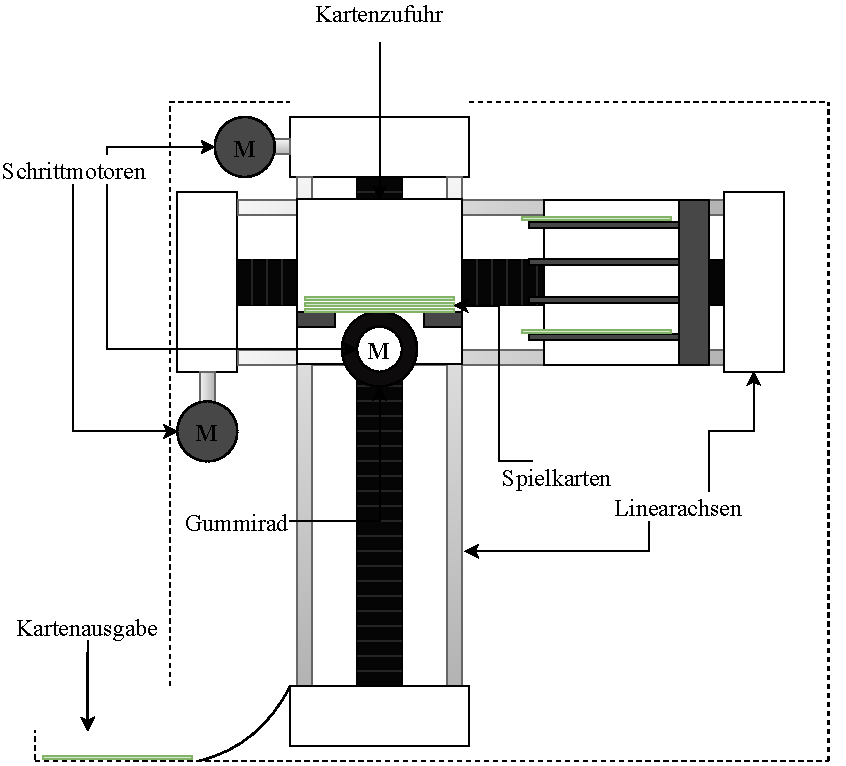
\includegraphics[scale=0.9,page=1]{fig/mech/Version1}
    \caption{Variante 1}
\end{figure}


Das erste Konzept würde mit zwei Linearachsen realisiert werden, diese wären im rechten Winkel zueinander
angeordnet. Die Senkrechte Linearachse ist mit einer Halterung versehen, diese Halterung ist in der Lage
ein Kartendeck aufzunehmen und die unterste Karte mithilfe eines Ausgaberades weiterzubefördern. Die zweite
Linearachse besitzt 4 Fächer, in der die Karten von der ersten Linearachsenausgabe zufällig befördert werden.
Dies wird realisiert, indem die erste Linearachse bei jeder Ausgabe zufällig das Fach durch hinauf und
hinabfahren wechselt. Befinden sich alle Karten im Lager, so fährt die erste Linearachse nach unten, danach
fährt die zweite Linearachse impulsiv nach links und bremst schlagartig ab, um die Karten aus dem Lager zu befördern. Diese fallen
Senkrecht in das Lager der ersten Linearachse, wo sie nun zum Ausgeben durch das Ausgaberad bereitliegen. \\



Durch die schnelle Bewegung der Linearachsen ist es möglich einen schnellen Mischprozess zu erreichen,
auch die Tatsache das es nur ein rotierendes Rad gibt und zwei Bewegliche Linearachsen führt dazu, das
Fehler bei Bewegungen nur selten Auftreten. Jedoch besteht durch den hohen Aufbau der Maschine und durch die hohe
Position der zweiten Linearachse die sich horizontal bewegt die Gefahr des Umkippens der Maschine, und somit ist
keine Stabilität mehr gegeben. Der Preis der Linearachsen ist ein weiterer Nachteil dieses Konzeptes, eine Linearachse
die unsere Anforderungen entspricht, wäre mit Motor und Schlitten zu teuer für unser Budget. \\

\textbf{Vorteile:}
\begin{itemize}
    \item schnelles Mischen
    \item wenige Fehlerquellen
\end{itemize}
\textbf{Nachteile:}
\begin{itemize}
    \item teuer
    \item großer Aufbau %Genaueres Beschreiben der Vor und Nachteile?
    \item instabil
\end{itemize}

\subsubsection{Variante 2 - Lagerrad mit Asugaberäder}

\begin{figure}[hb]
    \centering
    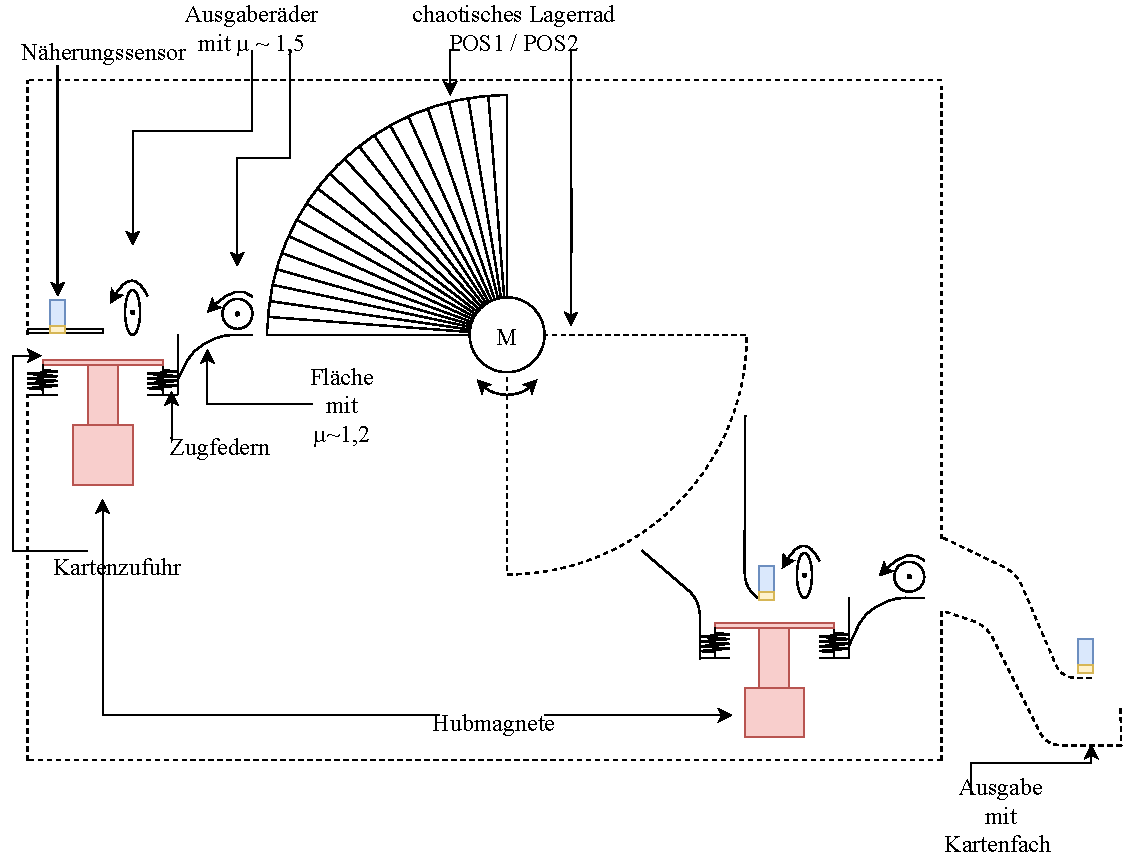
\includegraphics[scale=0.9,page=1]{fig/mech/Version2}
    \caption{Variante 2}
\end{figure}

Beim zweiten Konzept wird als Lager ein Viertel eines Zylinders benutzt. In diesem befinden
sich verschiedene Fächer, in der die Karten eingelagert werden. Dieser wird mit einem Motor betrieben
und dreht sich somit in die vorgegebenen Positionen um das Einlagern und das Ausgeben der Karten zu ermöglichen.
Die Karteneingabe erfolgt über einen Schlitz in der Frontplatte der Maschine, dort befindet sich ein Hubmagnet, der die Karten
zum weiterbefördern nach oben drückt. Ein Kapazitiver Sensor sorgt dafür, das sichergestellt werden kann, dass sich Karten auf dem Hubmagnet befinden.
Um eine Karte in das Lager zu befördern wird der Hubmagnet eingeschaltet und drückt das Kartendeck auf das erste Ausgaberad, um die Kraft des Hubmagnetes zu minimieren sind Zugfedern angebracht.
Das Ausgaberad befördert eine Karte weiter vor zum zweiten Ausgaberad, welches wiederum sicherstellt, das nur eine Karte in das Lagerrad transportiert wird.
Danach dreht das Lagerrad auf eine andere zufällig ausgewählte Position. Dieser Prozess wird so lange wiederholt, bis alle Karten des Kartendecks sich im Lagerrad befinden.
Befinden sich alle Karten im Lagerrad, so dreht sich dieses mit einer hohen Geschwindigkeit und wirft somit die Karten auf der Hinterseite der Maschine in eine Auffangführung. %Ist Geschwindigkeit der richtige Begriff? Eher Moment oder Drehzahl?
Diese Auffangsführung befördert die Karten in einen gleichen Mechanismus wie bei der Vorderseite der Maschine, in der sie von einem Hubmagneten nach oben gedrückt werden und von zwei Ausgaberädern zur
Kartenentnahme geschoben werden. Da die Karten zum Schluss nach einem Spielmodus und somit in einer bestimmten Anzahl ausgegeben werden, befindet sich ein Kapazitiver Sensor auch bei der Ausgabe der Karten,
dieser soll überprüfen, ob die Karten von dem Spieler bereits genommen wurden oder nicht.\\

Durch den niedrigen Aufbau der durch ein "Fließbandartiges" befördern der Karten erreicht wird, besitzt die Maschine ein hohes Maß an Stabilität, jedoch entsteht dadurch auch der Nachteil, dass die Maschine sehr lang wird. Da dieses
Konzept 5 bewegliche Räder besitzt, sowie zwei Hubmagneten, ist es anfällig für Fehler beim Bewegungsablauf. Auch kann nicht garantiert werden, dass nur eine Karte in das Lagerrad befördert wird, dies würde das Konzept des optimalen
Mischens zerstören. Die vielen Bauteile führen auch zu teureren Anschaffungskosten, die wir stark vermeiden möchten.\\

\textbf{Vorteile:}
\begin{itemize}
    \item stabil
    \item niedriger Aufbau
\end{itemize}
\textbf{Nachteile:}
\begin{itemize}
    \item lange Gesamtgröße
    \item viele bewegliche Bauteile / Fehlerquellen
\end{itemize}

\subsubsection{Variante 3 - Lagerrad mit Saugnäpfe}

\begin{figure}[H]
    \centering
    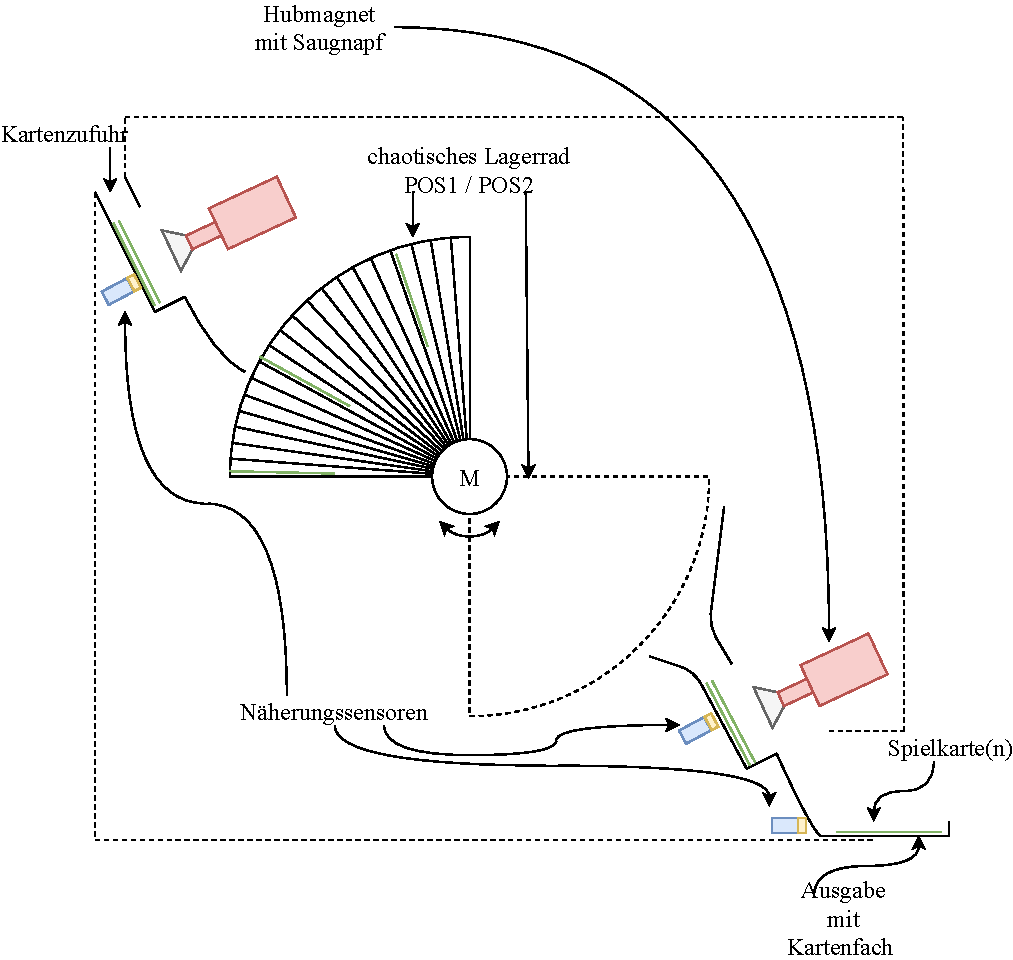
\includegraphics[scale=0.9,page=1]{fig/mech/Version3}
    \caption{Variante 3}
\end{figure}

Das dritte Konzept besitzt ein identes Lagersystem wie das zweite Konzept, ein Lagerrad, das in Fächer unterteilt ist und über einen Motor diverse Positionen einnehmen kann.
Das Kartendeck wird in den oberen / vorderen Anfang der Maschine eingeführt. Dort liegt, es schräg in einem Winkel von ca. 60°. Um sicherzustellen, dass sich Karten in dieser Halterung befinden
ist ein Kapazitiver Sensor an der Unterseite angebracht. Ein Hubmagnet der im rechten Winkel zu den Karten über der Halterung angebracht ist, saugt jede Karte einzeln an, indem ein Saugnapf, der an einem Hubmagneten
befestigt, ist heruntergedrückt wird. Ist die Karte angesaugt, so wird der Hubmagnet von einer Feder in seine Ausgangsstellung zurückgebracht, dabei wird die Spielkarte durch eine Platte abgestreift und fliegt somit in das Lager des
Lagerrades hinein. Dieser Prozess wird so lange wiederholt, bis sich alle Spielkarten des Kartendecks im Lagerrad befinden. Sind alle Karten im Lagerrad, so dreht sich dieses und wirft die Karten auf der Rückseite der Maschine in eine Führung, die die Karten in eine zweite Halterung befördern. Diese zweite Halterung ist ident aufgebaut wie die erste. Die Karten werden nun wieder einzeln vom Saugnapf angesaugt und in ein Ausgabefach am Ende der Maschine befördert. Im Ausgabefach befindet sich
ein Kapazitiver Sensor, dieser überprüft, ob die Karten vom Spieler bereits genommen wurden oder nicht.\\

Durch die wenigen Bauteile die dieses Konzept besitzt, nämlich zwei Hubmagnete und einen Motor, ist das Konzept wenig fehleranfällig bei Bewegungsabläufe. Außerdem ist es
durch die wenigen Bauteile im Vergleich billiger als die anderen Konzepte. Ein Problem dieses Konzeptes ist seine Höhe und dass das Lagerrad sich in der Mitte der Maschine befindet,
jedoch ist durch das geringe Gewicht des Lagerrades noch immer genügend Stabilität vorhanden, auch wenn sich dieses mit voller Geschwindigkeit dreht. \\

\textbf{Vorteile:}
\begin{itemize}
    \item billig
    \item wenig bewegliche Bauteile
\end{itemize}
\textbf{Nachteile:}
\begin{itemize}
    \item hocher Aufbau
\end{itemize}

 \subsection{Ausgaberäder}
Um die Karten weiterzubefördern werden bei zwei Konzepten Ausgaberäder benutzt, für diese gibt es verschiedene Konzepte dies sich in Preis, Herstellung und Funktionalität unterscheiden.\\
Das Ausgaberad ist mit einem Motor verbunden, dieses sorgt dafür das eine Karte von einem Kartendeck weiterbefördert wird.
\begin{itemize}
    \item \textbf{Rundes Ausgaberad}
\end{itemize}

\begin{figure}[H]
    \centering
    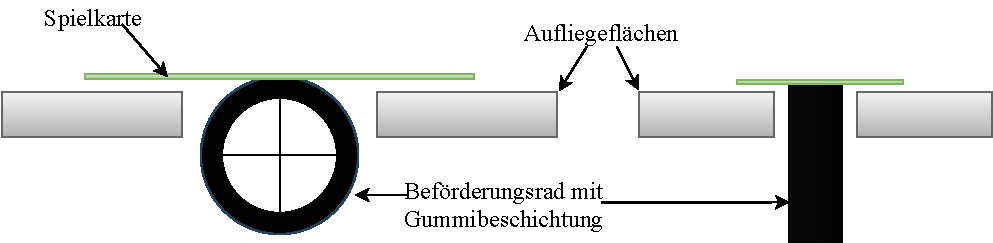
\includegraphics[scale=0.9,page=1]{fig/mech/RundesAusgaberad-Page-1}
    \caption{Rundes Ausgaberad}
\end{figure}

    Die einfachste Möglichkeit dieses Rad zu entwerfen, wäre ein einfaches rundes Ausgaberad. Dieses Rad wäre mit einer Schicht umhüllt, welche die Reibung
        dem Rad und der Karte erhöht. Das runde Rad wäre einfach zu fertigen und würde somit wenig kosten und nur einen geringen Zeitaufwand haben. Jedoch
        ist das Rad in der Lage mehr als nur eine Karte mit sich mitzuziehen, da es durchgehen Kontakt mit der Spielkartenoberfläche hat, dies hätte zur
        Folge, das mehrere Spielkarten zugleich weiterbefördert werden.
\begin{itemize}
    \item \textbf{Eliptisches Ausgaberad}
\end{itemize}

\begin{figure}[H]
    \centering
    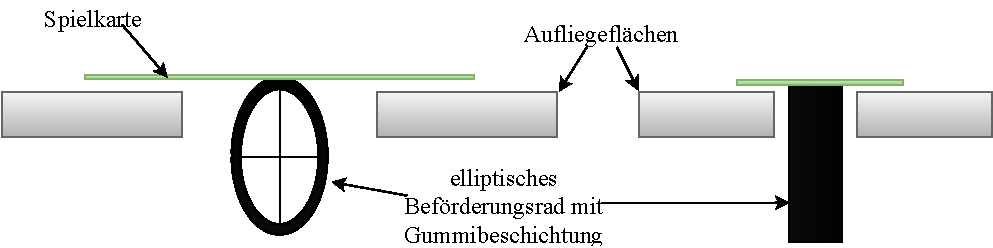
\includegraphics[scale=0.9,page=1]{fig/mech/ElliptischesAusgaberad}
    \caption{Eliptisches Ausgaberad}
\end{figure}


Ein elliptisches Ausgaberad wäre das nächste Konzept, dieses Rad wird auch wie beim ersten Rad mit einem Motor verbunden, um somit Karten zu befördern.
Durch die elliptische Form des Rades herrscht kein durchgehender Kontakt mit der Oberfläche der Spielkarte, aus diesem Grund ist die Chance das mehrere
Karten zugleich befördert werden minimiert. Jedoch setzt dies auch einen Motor voraus der in kurzer Zeit ein hohes Drehmoment entwickelt, da die
Karten schlagartig befördert werden. Das elliptische Rad würde in der Produktion auch mehr Kosten verursachen und wäre Zeitintensiver in der Herstellung. \\

\begin{itemize}
    \item \textbf{Vergleich der Ausgaberäder}
\end{itemize}

Da das primäre Ziel unserer Arbeit das perfekte Mischen der Spielkarten ist, wäre es besser das elliptische Ausgaberad in Betracht zu ziehen. Die Kosten
die durch die aufwendigere Herstellung entstehen wären überschaulich und somit wäre es von Vorteil dieses Konzept zu wählen. Durch die Tatsache, dass das elliptische Rad
das Kartendeck nur jede halbe Umdrehung berührt und nicht konstant, muss ein Motor für die Räder eingesetzt werden, der sich schnell genug dreht, um eine Karte mit einer Berührung
des Rades "herauszuschießen". Dies würde aber keine zusätzlichen Kosten verursachen. Aus diesen Gründen fällt die Wahl auf das \textbf{elliptisches Ausgaberad}. \\

\subsection{Klemmmechanissmen}
Um beim Ausgeben und beim Weiterbefördern der Karten die Chance zu minimieren das mehrere Karten auf einmal weiterbefördert werden, wird ein
Klemmmechanismus benutzt, dieser sorgt dafür das die Karten von außen Geklemmt werden, und somit nur die unterste Karte durch das Drehen des
Ausgaberades weiterbefördert wird.

\begin{itemize}
    \item \textbf{Primitiver Klemmmechanissmus}
\end{itemize}

\begin{figure}[H]
    \centering
    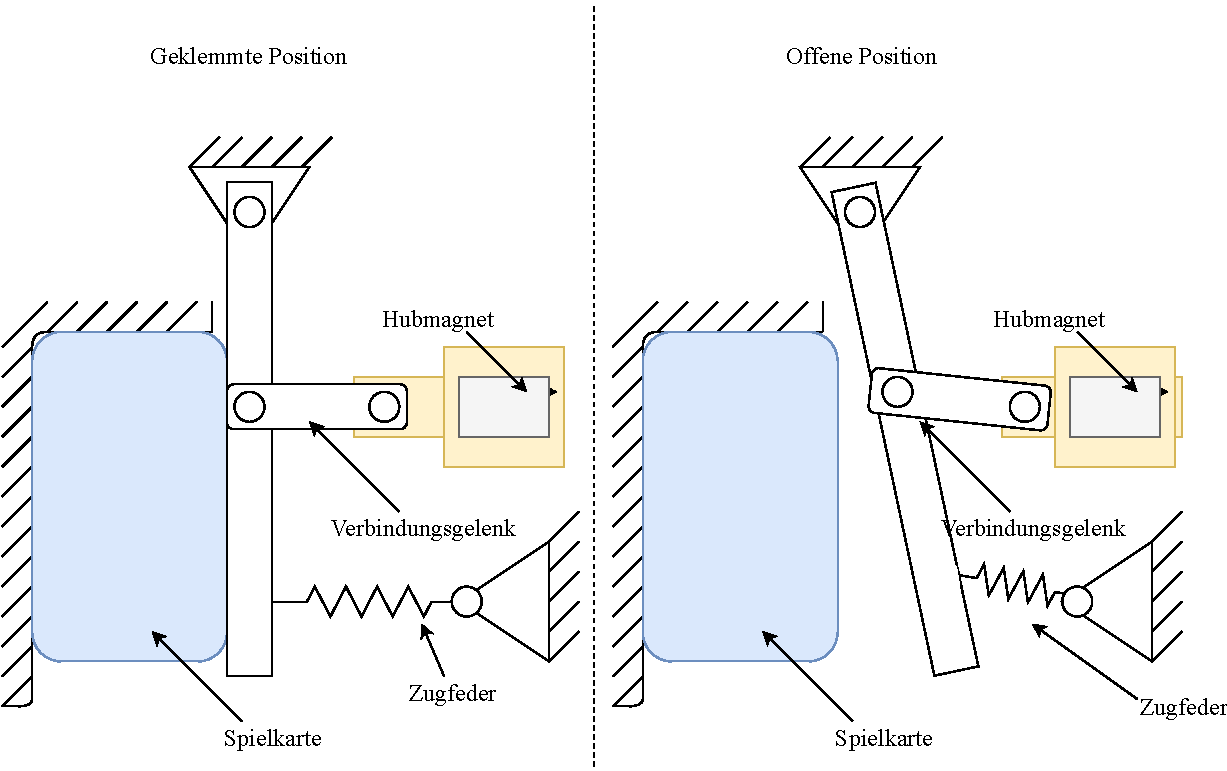
\includegraphics[scale=0.9,page=1]{fig/mech/Klemmmechanissmus1}
    \caption{Primitiver Klemmmechanissmus}
\end{figure}

Dieser Klemmmechanismus ist der primitivste und einfachste, dadurch aber auch der billigste. Die Karten werden auf der einen Seite an eine feste Wand gedrückt
auf der anderen Seite werden sie durch ein bewegliches Gelenk fixiert. Dieses Gelenk wird durch das Einschalten des Hubmagneten in die geschlossene Position bewegt,
soll das Gelenk wieder öffnen, so wird der Hubmagnet ausgeschaltet und eine Zugfeder zieht das Gelenk wieder in seine Ausgangsposition zurück.

\begin{itemize}
    \item \textbf{Komplexer Klemmmechanissmus}
\end{itemize}

\begin{figure}[H]
    \centering
    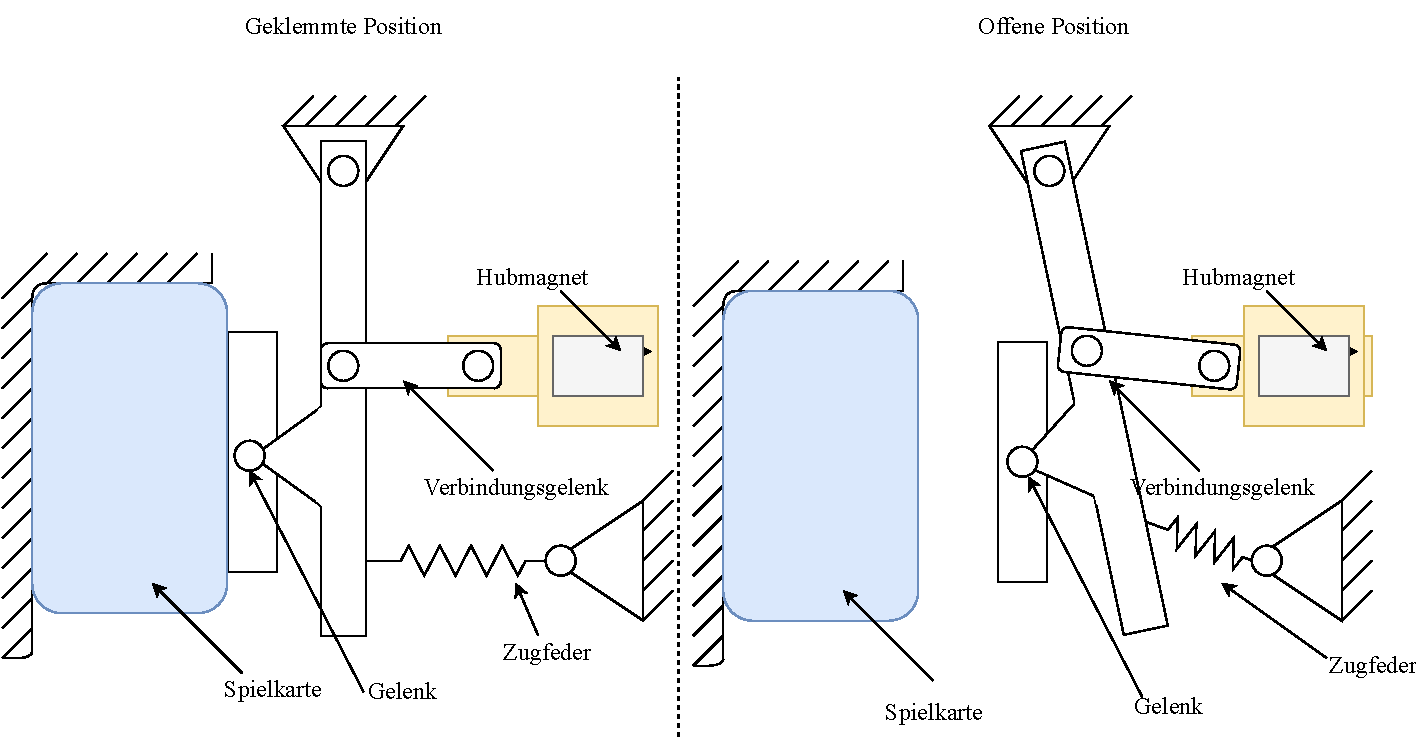
\includegraphics[scale=0.9,page=1]{fig/mech/Klemmmechanissmus2}
    \caption{Komplexer Klemmmechanissmus}
\end{figure}

Bei diesem Mechanismus werden die Karten auf der einen Seite durch eine feste Wand geklemmt, auf der anderen werden sie durch ein Gelenk geklemmt, dieses Gelenk
ist beweglich und gleicht somit verschiedene Kartengrößen aus. Um das Gelenk dieses Konzeptes zu schließen wird ein Hubmagnet benötigt, wird dieser eingeschalten
so schließt das Gelenk und passt sich der Kartengröße an. Soll es wieder geöffnet werden, so wird der Hubmagnet ausgeschaltet und eine Zugfeder bringt den Mechanismus wieder in den
Grundzustand. Dieses Konzept ist aufwendiger zu realisieren wie das erste, jedoch kann es verschiedene Kartengrößen klemmen und gleicht sich den Karten an. Das Konzept ist
dafür aber auch aufwendiger in der Produktion.

\begin{itemize}
    \item \textbf{Gummi Klemmmechanissmus}
\end{itemize}

\begin{figure}[H]
    \centering
    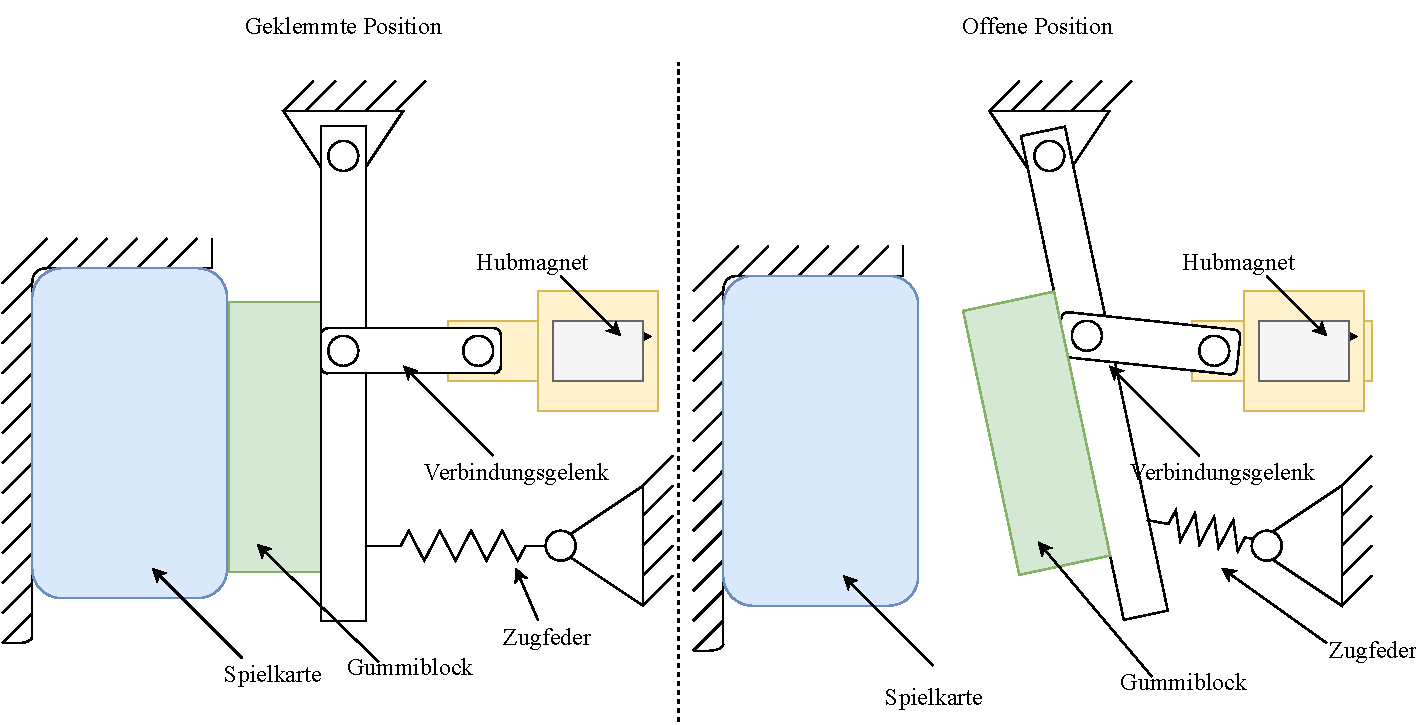
\includegraphics[scale=0.9,page=1]{fig/mech/Klemmmechanissmus3}
    \caption{Gummi Klemmmechanissmus}
\end{figure}

Der letzte Mechanismus ist funktionsmäßig gleich wie der primitive Klemmmechanismus, der einzige Unterschied besteht aus dem
Gummi-ähnlichen Block, der auf der Klemmfläche sitzt. Dieser soll sich den Karten anpassen und sorgt dafür das alle Karten gleichmäßig
geklemmt werden, auch erhöht es die Reibung zwischen den Karten und der Klemmoberfläche. Dieses Konzept wäre in der Herstellung vergleichsweise
einfach zu realisieren und dadurch auch billig in der Herstellung.


\begin{itemize}
    \item \textbf{Vergleich der Klemmmechanissmen}
\end{itemize}

Da alle Mechanismen die gleiche Anzahl an Bauteile erfordern, spielt der Preis bei dieser Auswahl keine große Rolle. Aus diesem Grund
sind die Kriterien Funktionalität und Aufwand in der Produktion. Der erst Mechanismus wäre der einfachste in der Produktion, jedoch
hat er durch sein nicht anpassungsfähiges Klemmgelenk Probleme mit verschiedenen Kartengrößen, aus diesem Grund fällt er bei diesem Auswahlverfahren durch.
Der zweite Mechanismus wäre der komplexe Klemmmechanismus, dieser würde sich zwar verschiedenen Kartengrößen anpassen, wäre aber etwas aufwendiger in der
Produktion und ist somit auch nicht die bevorzugte Wahl. Da er einfach in der Produktion ist und sich verschiedenen Kartengrößen anpassen kann, fällt die Wahl jedoch auf den Gummiklemmmechanismus.

\subsection{Seperation der Karten}
Da bei "Variante 3 - Lagerrad mit Saugnäpfe" Saugnäpfe mit Unterdruckprinzip in Verwendung kommen würden, liegt das Problem vor,
dass die Karten aneinander haften, dieses Problem entsteht durch den Unterdruck der beim Aufpressen des Saugnapfes entsteht.
Um zu garantieren, das nur eine Karte in das Lager befördert wird oder ausgegeben wird, müssen diese aneinander
haftende Karten getrennt werden.

\begin{enumerate}
    \item \textbf{Selbständiges Loslösen der Karten}\\
    Die billigste und primitivste Möglichkeit die Karten zu separieren wäre abzuwarten bis Luft zwischen den Karten von außen eindringt und alle Karten sich durch die Schwerkraft
    von der eigentlich angesaugten Karte getrennt haben. Jedoch zeigten Versuche die durchgeführt wurden, dass dies zu lange
    dauern würde und das Spielerlebnis somit beeinflussen würde.

    % Please add the following required packages to your document preamble:
    % \usepackage{multirow}
    \begin{table}[H]
        \centering
        \scalebox{0.9}{
        \begin{tabular}{|c|c|c|c|c|c|c|c|}
            \hline
            \textbf{}                         & \multicolumn{7}{c|}{\textbf{Sekunden}}                                                                  \\ \hline
            \multirow{21}{*}{\textbf{Karten}} &    & 1. Durchgang & 2. Durchgang & 3. Durchgang & 4. Durchgang & 5. Durchgang        & Mittelwert       \\ \cline{2-8}
            & 20 & 9.69         & 9.32         & 8.92         & 8.54         & 4.53                & 8.2              \\ \cline{2-8}
            & 19 & 9.1          & 9.97         & 13.82        & 6.71         & 7.75                & 9.47             \\ \cline{2-8}
            & 18 & 15.39        & 8.93         & 6.51         & 13.05        & 15.25               & 11.826           \\ \cline{2-8}
            & 17 & 6.45         & 6.67         & 6.16         & 8.06         & 6.97                & 6.862            \\ \cline{2-8}
            & 16 & 10.76        & 6.52         & 10.62        & 11.37        & 6.97                & 9.248            \\ \cline{2-8}
            & 15 & 12.81        & 6.45         & 16.22        & 8.74         & 4.7                 & 9.784            \\ \cline{2-8}
            & 14 & 3.46         & 9.78         & 11.72        & 5.85         & 6.39                & 7.44             \\ \cline{2-8}
            & 13 & 4.85         & 8.18         & 10.77        & 10.5         & 3.43                & 7.546            \\ \cline{2-8}
            & 12 & 15.1         & 5.37         & 12.36        & 8.54         & 12.31               & 10.736           \\ \cline{2-8}
            & 11 & 15.83        & 6.32         & 5.58         & 5.08         & 1.12                & 6.786            \\ \cline{2-8}
            & 10 & 7.14         & 8.4          & 11.21        & 12.76        & 4.43                & 8.788            \\ \cline{2-8}
            & 9  & 7.48         & 6.24         & 11.87        & 4.32         & 6.36                & 7.254            \\ \cline{2-8}
            & 8  & 4.68         & 5.65         & 8.61         & 5.2          & 4.41                & 5.71             \\ \cline{2-8}
            & 7  & 9.73         & 8.29         & 9.13         & 5.35         & 11.2                & 8.74             \\ \cline{2-8}
            & 6  & 5.41         & 5.16         & 8.05         & 4.98         & 9.73                & 6.666            \\ \cline{2-8}
            & 5  & 6.06         & 4.81         & 7.8          & 4.73         & 7.19                & 6.118            \\ \cline{2-8}
            & 4  & 4.86         & 9.87         & 7.74         & 9.51         & 7.4                 & 7.876            \\ \cline{2-8}
            & 3  & 4.54         & 11.31        & 4.31         & 6.74         & 10.82               & 7.544            \\ \cline{2-8}
            & 2  & 4.83         & 2.19         & 4.13         & 3.78         & 5.71                & 4.128            \\ \cline{2-8}
            &    &              &              &              &              & \multicolumn{2}{c|}{Mittelwert: 7.932} \\ \hline
        \end{tabular}}
        \caption{Tabelle Haftzeit der Karten}
        \label{tab:my-table}
    \end{table}

    \begin{figure}[H]
        \centering
        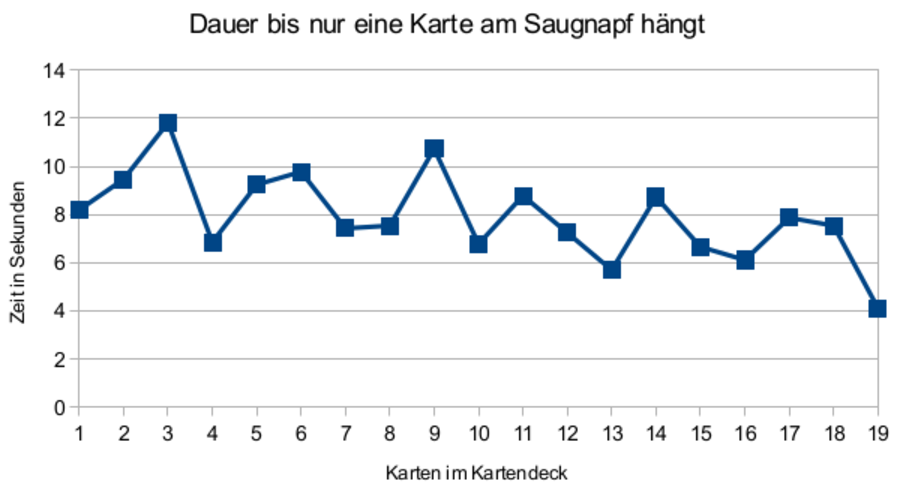
\includegraphics[scale=1,page=1]{fig/mech/Haftzeit}
        \caption{Diagramm Haftzeit der Karten}
    \end{figure}

    Wie man in Tabelle 1.1 und in Abbildung 1.9 erkennen kann dauert es im Durchschnitt 7,932 Sekunden bis sich nur mehr die
    eigentlich angesaugte Karte am Saugnapf befindet. Der Versuch wurde mit 1Kg Ansaugdruck durchgeführt. Es gab insgesamt
    5 Durchgänge, auch wurden alle Möglichkeiten der Kartenanzahl im Kartendeck berücksichtigt, so saugte der Saugnapf
    bei der ersten Durchgangsreihe die erste Karte an, die auf 19 anderen Karten liegt, bis hin zu einem Saugnapf, der
    eine Karte ansaugt, die nur auf einer einzelnen anderen Karte liegt.

    \textbf{Vorteile:}
    \begin{itemize}
        \item billig
        \item keine zusätzlichen Bauteile benötigt
    \end{itemize}
    \textbf{Nachteile:}
    \begin{itemize}
        \item lange Wartezeit
        \item unzuverlässig
    \end{itemize}

    \item \textbf{Rütteln}\\\\
Ein weiteres Konzept um die angesaugte Karten von den anderen zu trennen wäre die Karten minimal zu rütteln.
Da die angesaugte Karte viel stärken an dem Saugnapf haftet als die Karten, die nur an der angesaugten Karten haften,
könnte der Hubmagnet oder der Ansaugmechanismus leicht gerüttelt werden, so würden die anderen Karten schneller den
Unterdruck untereinander verlieren und sich somit schon in kurzer Zeit separieren lassen. Jedoch müsste für dieses Konzept
ein Mechanismus entwickelt und produziert werden der nur einen ausgewählten Bereich rüttelt, dies wäre mit weiteren Bauteilkosten und
Aufwand verbunden.

\textbf{Vorteile:}
\begin{itemize}
    \item zuverlässig
\end{itemize}
\textbf{Nachteile:}
\begin{itemize}
    \item teurer
    \item zusätzliche Bauteile
    \item zusätzliche Größe
\end{itemize}



    \item \textbf{Abstreifbürsten}\\


Bei diesem Konzept sind bürstenartige Abstreifvorrichtungen in der Kartenhalterung angebracht. Diese Bürsten sollen beim Aufheben der
angesaugten Karte die anderen Karten die mitgehoben wurden abstreifen. Dabei ist es wichtig, dass die Bürste den richtigen Widerstand aufbringt.
Ist der Widerstand zu hoch, wird auch die eigentlich angesaugt Karte mit abgestreift, ist er jedoch zu niedrig ist es möglich, dass die anderen Karten
die mitgehoben werden nicht abgestreift werden.

\textbf{Vorteile:}
\begin{itemize}
    \item zuverlässig
    \item billig
\end{itemize}
\textbf{Nachteile:}
\begin{itemize}
    \item Karten werden seitlich abgenützt
    \item komplizierter Einbau
\end{itemize}

\begin{figure}[H]
    \centering
    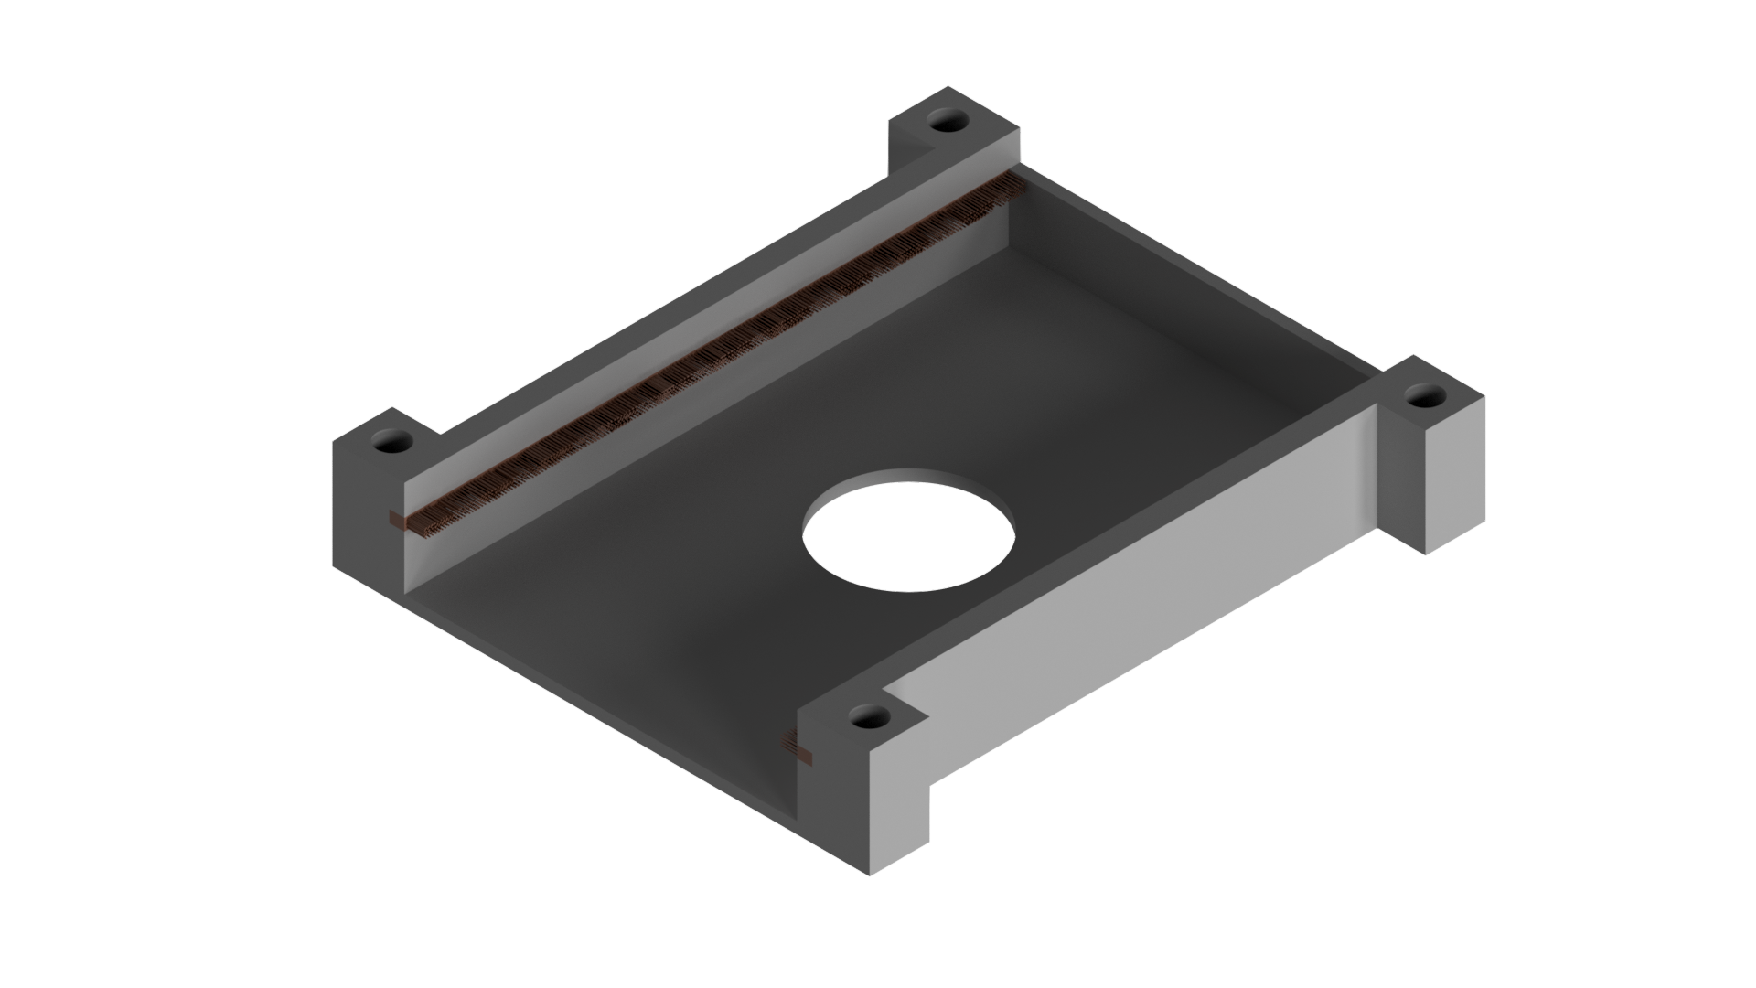
\includegraphics[scale=0.5,page=1]{fig/mech/AusgabeMitBuersten}
    \caption{Ausgabe mit Bürsten}
\end{figure}

    \item \textbf{Gummiabsstreifer}\\

Dieses Konzept funktioniert ähnlich wie das "Abstreifbürsten Konzept". Es besitzt seitlich Abstreifplatten die aus Gummi sind, diese
sollen der angesaugten Karte helfen, die mitgezogenen Karten abzustreifen. Wie beim vorherigen Konzept muss hierbei das Gummi auch so
dimensioniert werden, dass es einerseits nicht zu steif ist und die eigentlich angesaugt Karte abstreift, andererseits sollte es steif genug sein, um die Karten die mitgehoben werden abzustreifen. Man die Steifigkeit des Gummistreifens verändern, indem man die Breite der Einschnitte
erhöht oder vermindert.

\begin{figure}[H]
    \centering
    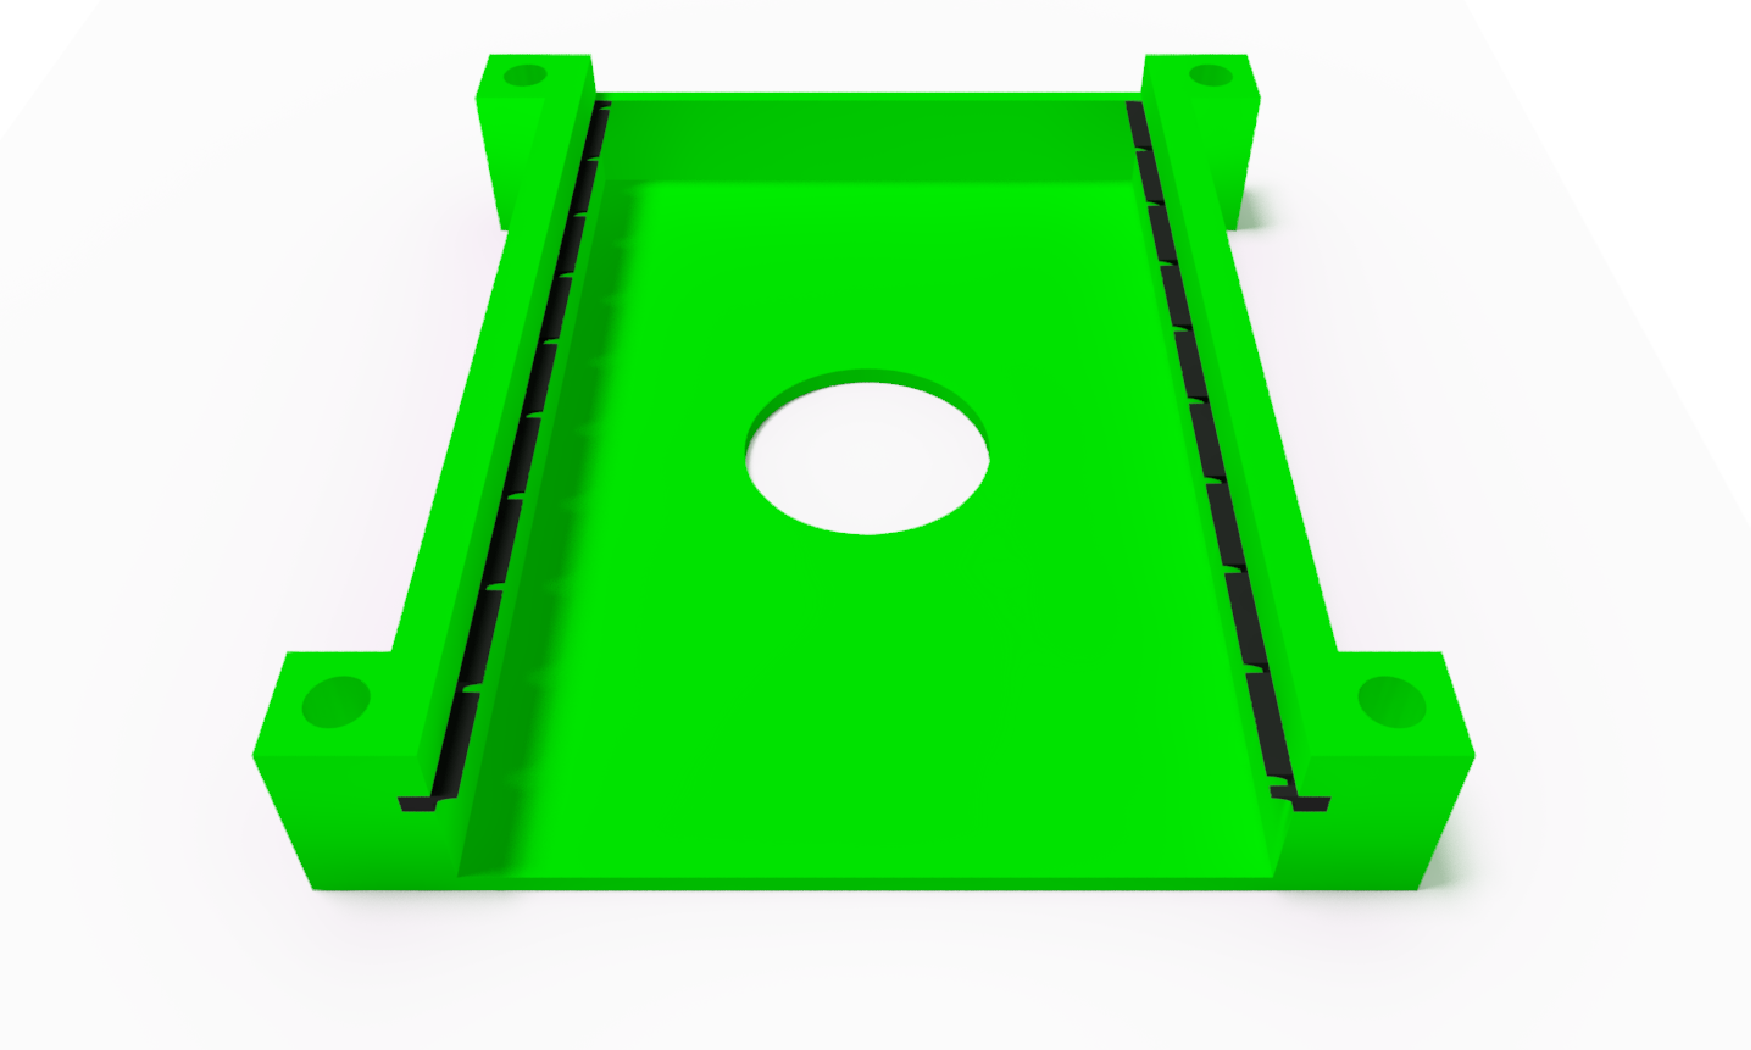
\includegraphics[scale=0.5,page=1]{fig/mech/AusgabeMitGummiabstreifer}
    \caption{Ausgabe mit Gummiabsstreifer}
\end{figure}

\textbf{Vorteile:}
\begin{itemize}
    \item zuverlässig
    \item billig
\end{itemize}
\textbf{Nachteile:}
\begin{itemize}
    \item Gummi wird spröde
\end{itemize}
\end{enumerate}

\subsection{Saugmechanismus}

Da bei der 3. Variante, Lagerrad mit Saugnäpfe, Saugnäpfe zum Einsatz kommen, muss entschieden werden, welche Saugnäpfe angewandt werden.

\begin{itemize}
    \item \textbf{einfacher unterdruck Saugnapf}
\end{itemize}
Die erste Möglichkeit wäre einen einfachen Saugnapf zu nehmen, der durch Anpressen an einer Oberfläche einen Unterdruck erzeugt und somit haftet. Ein Vorteil dieses Saugnapfes ist es, dass es kostengünstig ist und keine weiteren Bauteile benötigt sowie die
unkomplizierte Befestigung an dem Hubmagneten über ein Gewinde.
Jedoch muss dieser Saugnapf mit einer gewissen Kraft auf das Kartendeck gepresst werden, um einen Unterdruck erzeugen zu können. Dies kann dazu führen, dass zwischen den Karten auch ein Unterdruck erzeugt wird und somit mehr als eine Karte vom Saugnapf
hochgehoben wird. Ein weiterer Nachteil wäre, das die Karte nicht steuerbar abwerfbar ist, da sie erst abfällt, wenn der Unterdruck verschwindet. Dies kann zu unerwarteten Wartezeiten führen. Wenn der Ansaugdruck durch den Hubmagneten nicht erreicht wird, kann
es auch dazu führen, dass keine Karte angesaugt wird. Dies kann die Wartezeiten wiederum verlängern und somit den Spielablauf stören.

\textbf{Vorteile:}
\begin{itemize}
    \item Billig
    \item unkomplizierter Einbau
\end{itemize}
\textbf{Nachteile:}
\begin{itemize}
    \item unzuverlässig
\end{itemize}

\begin{itemize}
    \item \textbf{Vakuumsaugnapf}
\end{itemize}
Eine andere Möglichkeit wäre ein Vakuumsaugnapf, dieser erzeugt seinen Unterdruck über eine Vakuumpumpe und kann somit gesteuert werden. Der Vorteil dieses Saugnapfes ist es, dass die Karten zu einer gewünschten Zeit abgeworfen werden können, da man den
Unterdruck des Saugnapfes durch die Pumpe steuern kann. Ein anderer Vorteil ist, dass der Hubmagnet keine hohe Kraft aufweisen muss, da der Saugnapf nicht mehr auf die Karten aufgepresst werden muss, dies würde auch das Problem, dass mehrere Karten auf einmal
aufgehoben werden, lösen. Der Nachteil dieser Möglichkeit wäre jedoch der erhöhte Preis des Saugnapfes sowie die zusätzlichen Bauteile, wie zum Beispiel die Pumpe und die Valve. Außerdem ist der Einbau des Saugnapfes etwas komplizierter, da ein Luftdruckschlauch
zum Saugnapf geführt werden muss.

\textbf{Vorteile:}
\begin{itemize}
    \item Zuverlässig
    \item Unterdruck ist kontrollierbar
\end{itemize}
\textbf{Nachteile:}
\begin{itemize}
    \item mehr Bauteile
    \item teuer
    \item komplizierter Einbau
\end{itemize}

\begin{itemize}
    \item \textbf{Vergleich der Saunäpfe}
\end{itemize}

Beide Saugnäpfe würden ihre individuellen Vorteile besitzen. Da wir zum einen ein begrenztes Budget haben wäre der einfache Unterdrucksaugnapf für uns attraktiv, zum anderen wäre der Vakuumsaugnapf durch seine Zuverlässigkeit von Vorteil.
Da der ausgewählte Hubmagnet jedoch nicht in der Lage ist, den erforderlichen Ansaugdruck zu erreichen, und das kontrollierte Abwerfen der Karten maßgeblich für die Funktion der Maschine ist, fällt unsere Auswahl auf den \textbf{Vakuumsaugnapf}.
\subsection{Endauswahl der Varianten}

\textbf{\large{Gegenüberstellung der Varianten}}

\begin{table}[H]
\centering
\scalebox{0.8}{
    \begin{tabular}{|c|c|c|ll}
        \cline{1-3}
        \textbf{Variante}             & \textbf{Vorteile}                                                                & \textbf{Nachteile}                                                                                    &  &  \\ \cline{1-3}
        1 - Linearachsen              & \begin{tabular}[c]{@{}c@{}}schnelles Mischen\\ wenige Fehlerquellen\end{tabular} & \begin{tabular}[c]{@{}c@{}}teuer\\ großer Aufbau\\ instabil\end{tabular}                              &  &  \\ \cline{1-3}
        2 - Lagerrad mit Ausgaberäder & \begin{tabular}[c]{@{}c@{}}stabil\\ niedriger Aufbau\end{tabular}                & \begin{tabular}[c]{@{}c@{}}lange Gesamtgröße\\ viele Bewegliche Bauteile / Fehlerquellen\end{tabular} &  &  \\ \cline{1-3}
        3 - Lagerrad mit Saugnäpfe    & \begin{tabular}[c]{@{}c@{}}billig\\ wenig bewegliche Bauteile\end{tabular}       & hoher Aufbau                                                                                          &  &  \\ \cline{1-3}
    \end{tabular}}
    \caption{Vergleich der Varianten}
\end{table}

\textbf{\large{Begründung der Wahl}}\\
Alle drei Varianten wurden durchdacht und bieten ihre individuellen Vorteile. Durch den enormen Preis von
Variante 1 ist diese aber nicht für unser Projekt geeignet. Das optimale Konzept des Mischens wird am besten durch
Variante 3 realisiert, da diese die niedrigste Wahrscheinlichkeit aufweist, mehrere Karten auf einmal in das Lager zu befördern.
Da Variante 3 im Vergleich zur Variante 2 weniger Bauteile besitzt, ist diese Variante sowohl Preislich ansprechender für uns
sowie auch die Tatsache das Fehlerquellen durch bewegliche Bauteile minimiert werden. \\
Somit fällt die finale Wahl auf \textbf{Variante 3}.



\pagebreak
\section{Konstruktion}
\subsection{Konstruktion des Lagerrades}
Das Lagerrad soll durch das zufällige Rotieren das Mischen der Karten ermöglichen. Im Verlauf der Diplomarbeit wurde das Lagerrad mehrfach überarbeitet.
Die grundsätzliche Form dieses Rades besteht aus einem Viertel eines Hohlzylinders, der in mehrere Fächer unterteilt ist. Die erste Version dieses Rades besaß 20 Unterteilungen.

\begin{figure}[H]
    \centering
    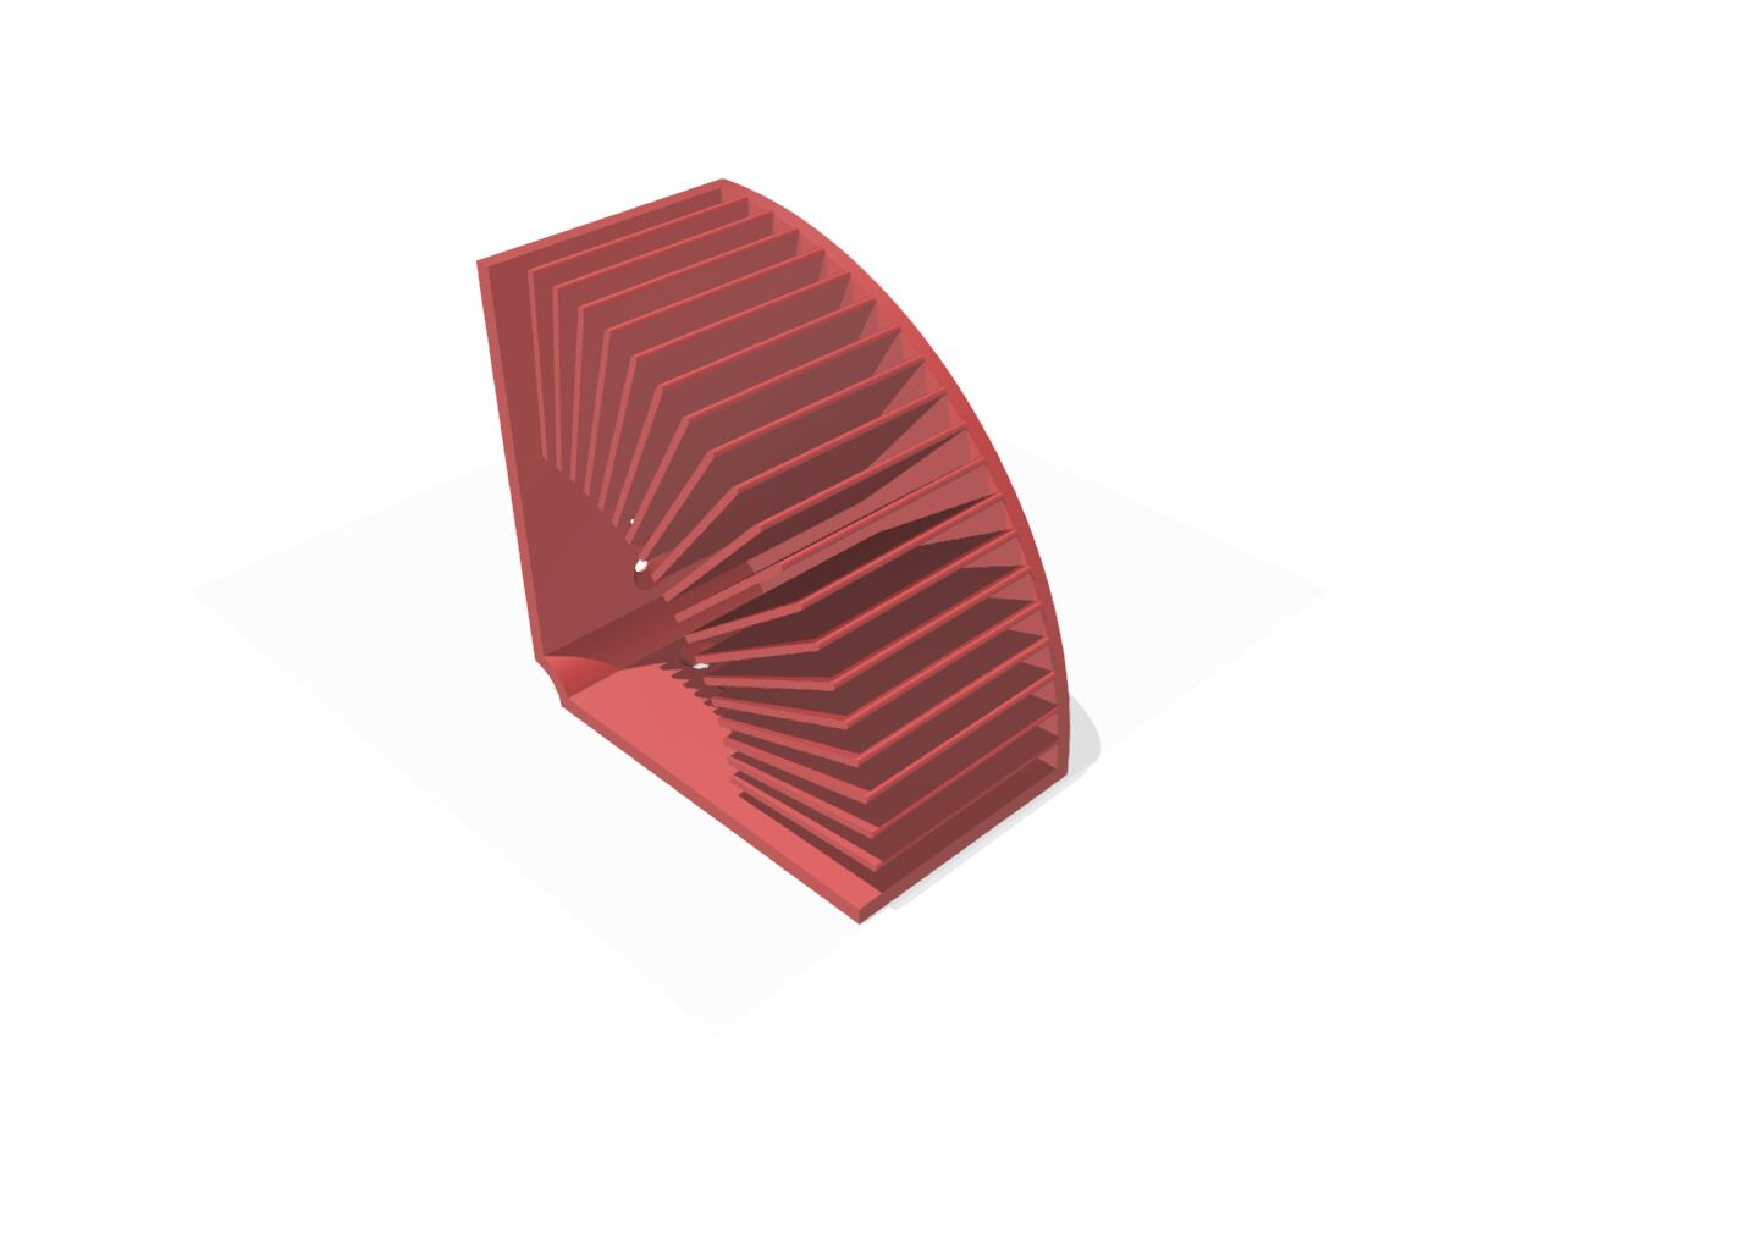
\includegraphics[scale=0.5,page=1]{fig/mech/LagerRad20F}
    \caption{Version 1: Lagerrad 20 Fächer (geöffnete Außenwand zur vereinfachten Ansicht)}
\end{figure}

In der oben angezeigten Grafik wurde die Außenwand entfernt, um eine bessere Einsicht in das Bauteil zu bekommen.
Durch die 20 Unterteilungen muss der Schrittmotor genauere Positionen anfahren, außerdem wäre der Aufwand beim Produzieren groß. Aus diesem Grund
entschieden wir uns die Unterteilungen zu minimieren und kamen zu dem Entschluss, dass 4 Unterteilungen für ein optimales Mischen ausreichen. Diese Konstruktion
wurde nach einem Stecksystem entworfen, sodass man die einzelnen Teile herstellen kann und diese danach zusammenstecken und verkleben kann.

\begin{figure}[H]
    \centering
    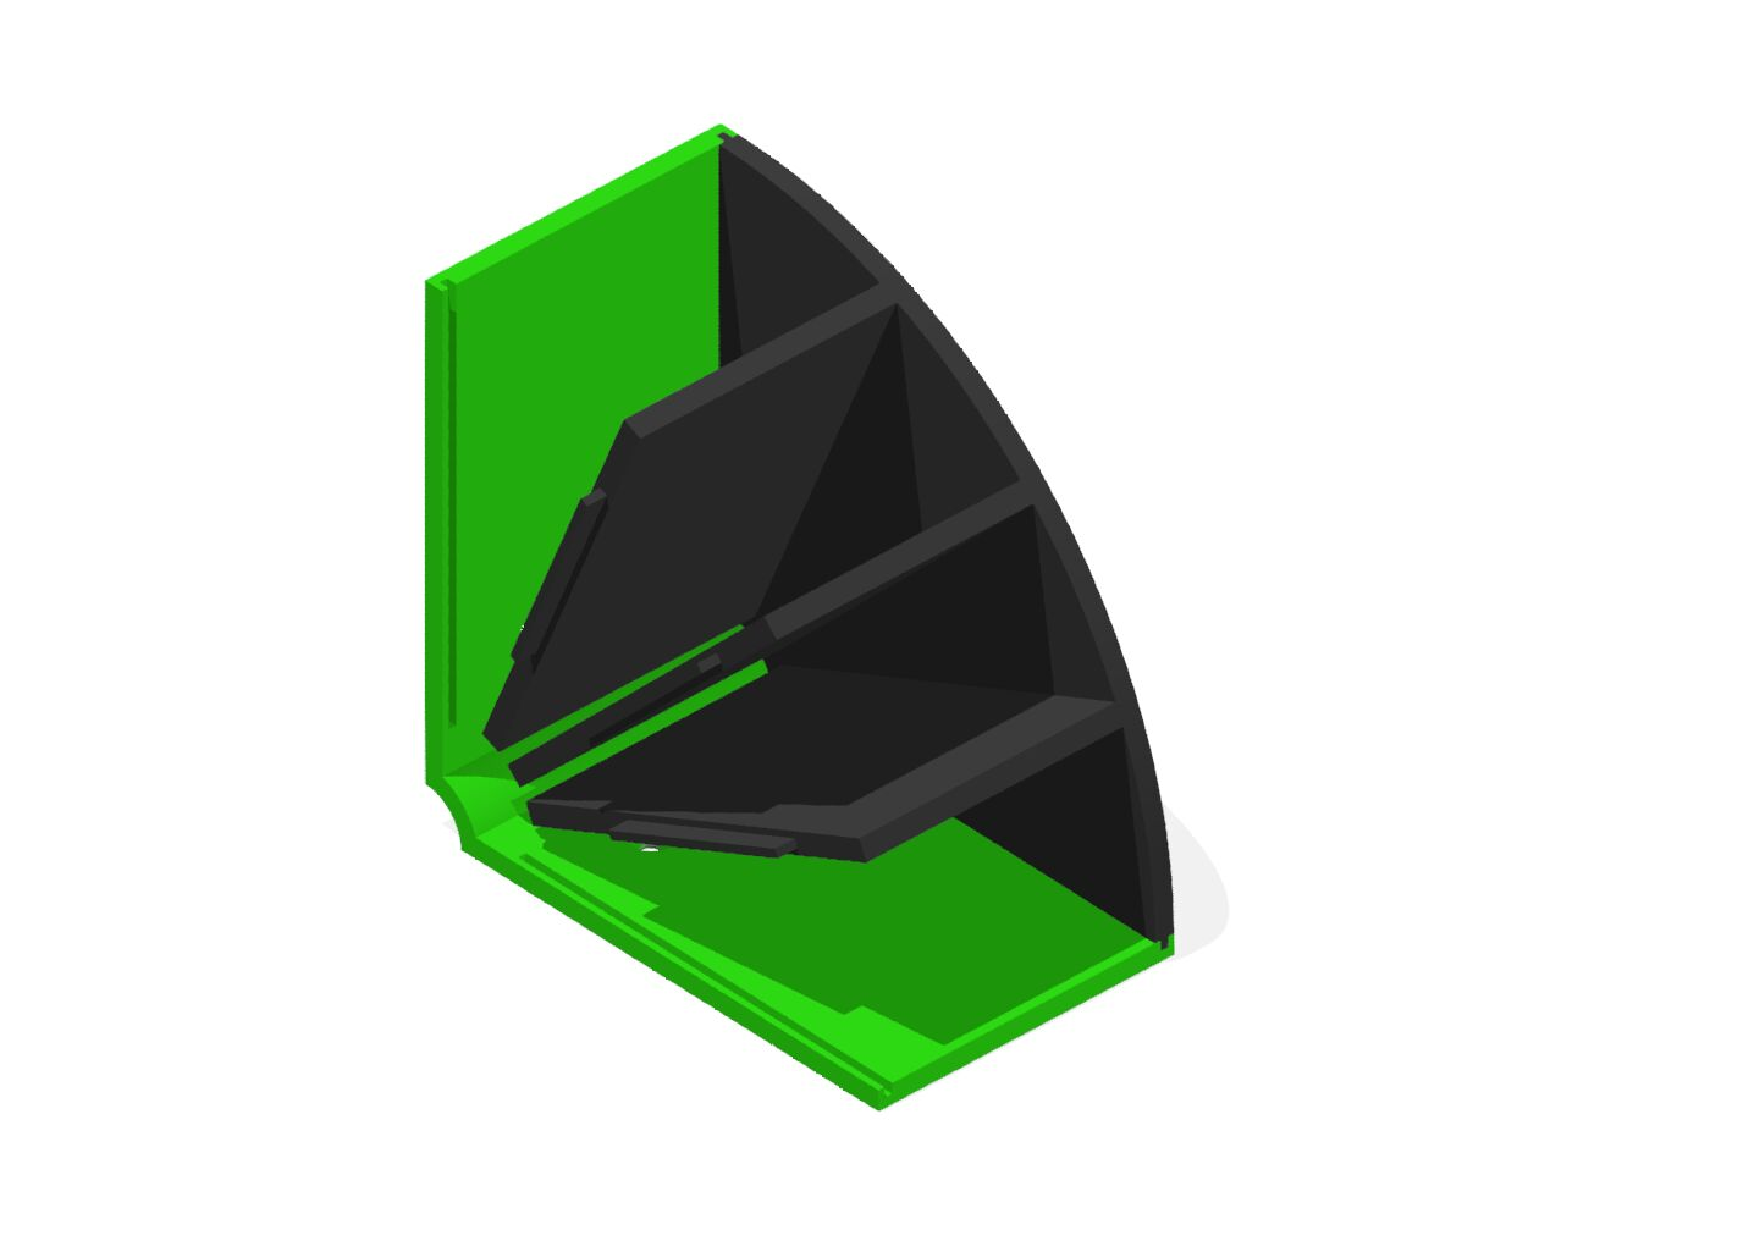
\includegraphics[scale=0.5,page=1]{fig/mech/LagerRad4F}
    \caption{Version 2: Lagerrad 4 Fächer (geöffnete Außenwand zur vereinfachten Ansicht)}
\end{figure}


Auch in der oben gezeigten Grafik wurde die Außenwand entfernt, um das Bauteil besser zu veranschaulichen.
Das Lagerrad besteht aus mehreren Einzelteilen:

\subsubsection{Außenwände}
Die Außenwände wurden in der Form eines Teiles eines Kreises konstruiert und geben somit die Form des Lagerrades vor. Sie besitzen jeweils 2 Laschen an der äußeren Seite, diese verbinden die Außenwände später mit den Seitenwänden des Lagerrades.
Außerdem besitzen sie jeweils 3 Ausfräsungen auf ihrer Grundfläche, über die sie später mit den Trennplatten versteckt werden. Bei der Konstruktion der Ausfräsungen ist dabei zu achten, dass sie etwas größer als benötigt gezeichnet werden, da bei der
Fertigungsart des 3D-Druckens Innenbohrungen und Innenfräsungen durch die Ungenauigkeit des Druckers kleiner gedruckt werden. Wie auch bei den Innenfräsungen müssen die Laschen auf der Außenseite etwas kleiner konstruiert werden, da diese wiederum beim
Drucken größer gedruckt werden, als sie ursprünglich gezeichnet wurden.

\subsubsection{Seitenwände}
Diese Bauteile verbinden das Lagerrad mit dem Lagerradhalterungsmodul. Sie besitzen auf der äußeren Seite der Grundfläche
jeweils 2 Auskerbungen. Über diese werden sie mit den Laschen der Außenwände verbunden. Um einen Durchgang für die Welle zu schaffen,
schließen die Bauteile auf der unteren Seite nicht im rechten Winkel ab, sondern sind nach innen radial abgerundet.
Je Bauteil sind 2 Bohrungen vorhanden, über diese wird es mit dem Lagerradhalterungsmodul verbunden.
Die Bohrungen sind als Senklochbohrungen ausgeführt, da somit die Schraube komplett in das Bauteil versenkt werden kann
 und das Hineinrutschen der Karten in das Lagerrad nicht behindert wird.

\subsubsection{Trennplatte}
Um die einzelnen Lagerfächer zu unterteilen, ist die Trennplatte konstruiert worden. Dieses Bauteil ist ein einfacher
Quader mit je 2 Laschen an den Außenseiten. Diese Laschen werden mit den Ausfräsungen der Außenplatte versteckt.
Hierbei ist wieder zu achten, dass die Laschen kleiner konstruiert werden, da sie durch den 3D-Druck an Größe zunehmen
werden.

\subsection{Konstruktion des Lagerradhalterungsmoduls}
Um das Moment der Welle effektiv von der Welle zum Rad zu übertragen, wurde ein Lagerradhalterungsmodul entworfen. Dieses Modul wird
benötigt, da das Wellenmoment nicht effektiv an einem 3D-gedruckten Bauteil angreifen kann, da das gedruckt PLA
die kontinuierlichen Richtungswechsel sowie das abrupte Bremsens des Motors in Kombination mit der
Trägheit des Lagerrades nicht standhalten würde. Dieses Modul besteht aus folgenden Einzelteilen:

\subsubsection{L-Grundplatte}
Dieses Bauteil, siehe Abbildung ......., verbindet die Motorwelle sowie die Lagerwelle mit der Verbindungsplatte und somit auch das Lagerrad.
Es überträgt somit auch das Moment des Motors. Es besitzt je 4 Bohrungen mit Zylinderschraubensenkungen, über die sie mit
der Verbindungsplatte verbunden wird. Außerdem besitzt sie eine Bohrung mit einer Querbohrung. Über diese werden die
Wellen geführt und mit einer Schraube am Bauteil fixiert.
Dieses Bauteil wurde ursprünglich aus Aluminium gefertigt, durch Versuche mit einer 3D-gedruckten L-Grundplatte zeigte
sich jedoch, dass diese sich genauso gut eignet und optisch ansprechender ist. Um nicht in Konflikt mit dem Lagerrad
zu stehen, hat das Bauteil jeweils 2 Ausbuchtungen nahe der Welle.

\subsubsection{Verbindungsplatte}
Die Verbindungsplatte nimmt das von der L-Grundplatte aufgenommene Moment des Motors und überträgt es an das Lagerrad weiter.
Sie wurde als einfacher Aluminiumquader konstruiert und besitzt insgesamt 6 Bohrungen. Zwei Bohrungen sind auf der
Grundfläche des Bauteils und besitzen ein Gewinde. Diese verbinden das Lagerradhalterungsmodul mit dem Lagerrad. Je 2
Bohrungen sitzen auf der Unterseite sowie auf der Oberseite der Verbindungsplatte und sind ebenfalls mit Gewinde
ausgeführt, durch diese Gewindebohrungen wird das L-Bauteil mit der Verbindungsplatte verbunden.
Dieses Bauteil wurde aus Aluminium gefertigt, da es problematisch ist ein Gewinde in PLA zu schneiden, außerdem spielt
das zusätzliche Gewicht des Aluminiums bei diesem Modul nur eine geringe Rolle.

\subsubsection{Motorwelle}
Um das Moment vom Motor auf die L-Grundplatte zu übertragen, wird die Motorwelle benötigt. Diese ist eine einfache Welle
mit einer Gewindebohrung am äußeren Ende der Welle. Diese dient dazu, die Welle mit der L-Grundplatte zu verbinden.
Am anderen Ende ist die Welle über die Kupplung mit dem Motor verbunden.
Die Welle wurde an der Drehbank gefertigt und anschließend an der Fräsmaschine die Gewindebohrung gebohrt.

\subsubsection{Lagerwelle}
Die Lagerwelle unterscheidet sich von der Motorwelle lediglich durch ihre Länge. Sie wird auf der einen Seite mit der
L-Grundplatte verschraubt, auf der anderen Seite wird sie mit dem Zweiloch-Flanschlager auf der Vorderseite des Gehäuses über
2 Wurmschrauben geklemmt.

\begin{figure}[H]
    \centering
    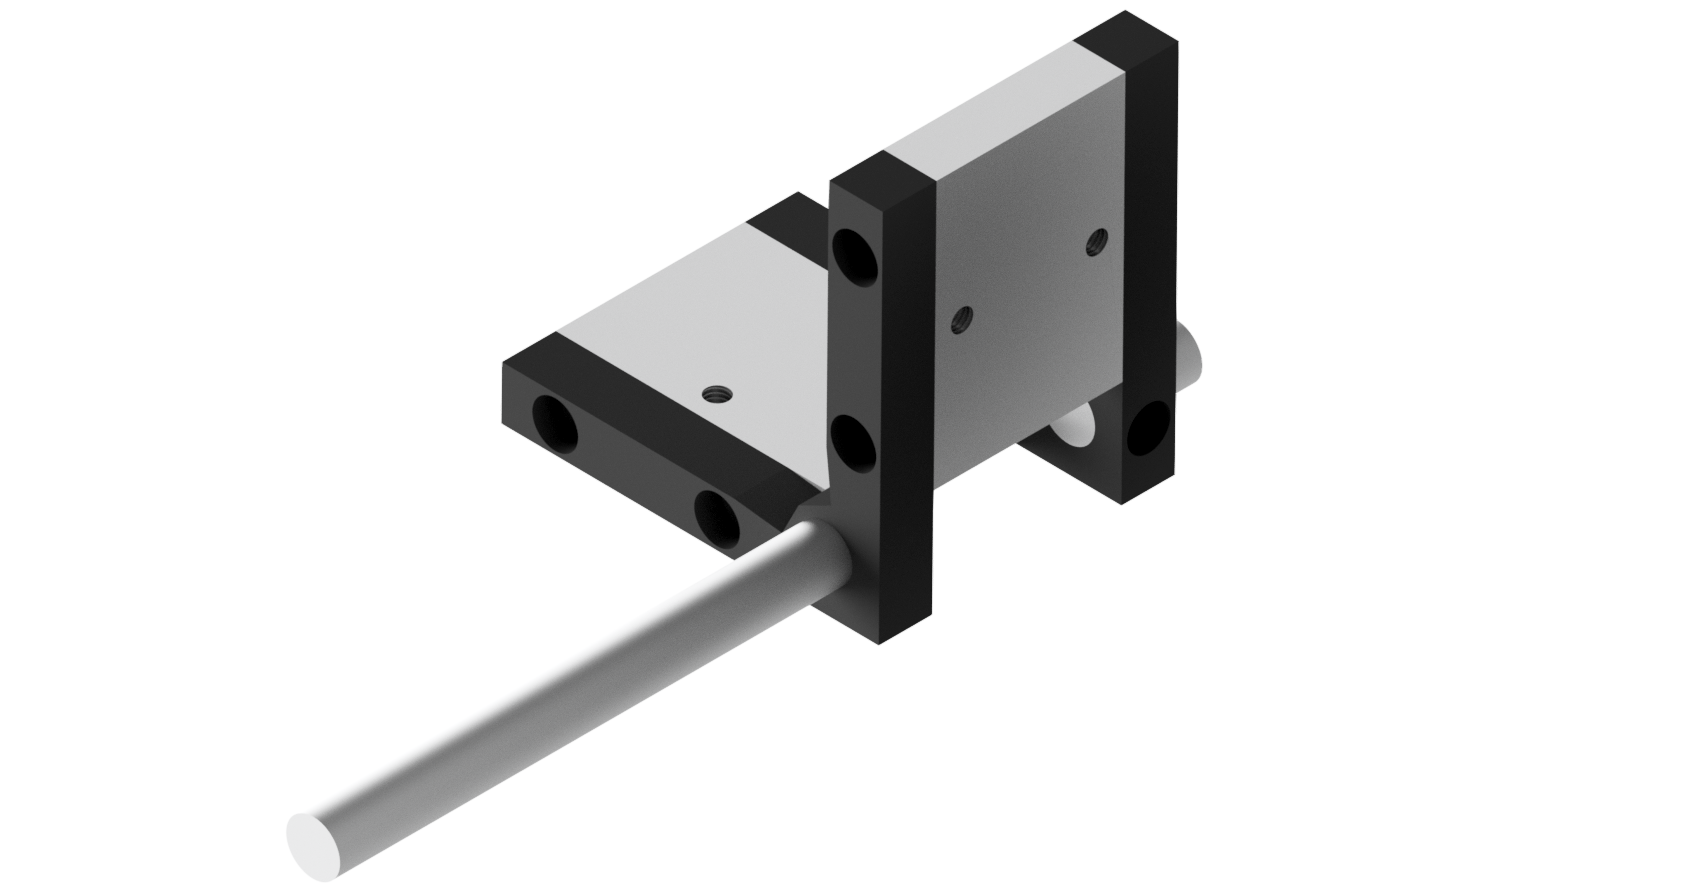
\includegraphics[scale=0.25,page=1]{fig/mech/LagerRadGruppekomplett}
    \caption{Lagerradhalterungsmodul}
\end{figure}

\subsection{Konstruktion der Motorhalterungsgruppe}

Die Motorhalterung, siehe Abbildung ......, hat den Zweck den Motor an das Gehäuse zu befestigen und ihn somit für die Welle auszurichten. Der ausgewählte Schrittmotor
besitzt eine mitgelieferte Montagehalterung die mit 4 Schrauben an den Motor geschraubt wird. Die Motorhalterung entspricht dem Nema 17
Standard und ist somit universal für Motoren dieser Norm anwendbar. Die Motorhalterung wird mittels 2 Schrauben an einen verzinkten Edelstahlwinkel angeschraubt, ist aber
in der Position noch Einrichtbar. Der Winkel wird über 4 Schrauben mit dem Gehäuse aus Polycarbonat verschraubt.

\subsection{Konstruktion des Kartenhalterungsmodul}
Die Karten müssen nach dem Einführen in die Maschine und nach dem Auswerfen aus dem Lagerrad zwischengelagert werden, da sie
von dem Hubmagneten und dem Saugnapf einzeln aufgehoben und ausgegeben werden. Für diese Aufgabe kommt das Modul der
Kartenhalterung, siehe Abbildung ...., zum Einsatz. Dieses Modul muss sicherstellen, dass genug Platz für mindestens 20 gewöhnliche Spielkarten  mit den Maßen 100 x 66
vorhanden ist. Das Modul besteht aus mehreren einzelnen Bauteilen:

\subsubsection{Sensorhalterung}
Die Sensorhalterung, siehe Abbildung ...., dient dazu den kapazitiven Sensor zu befestigen. Dieser wird mithilfe zwei Muttern und zwei Sicherungsringen
über das Gewinde des Sensors befestigt. Durch diese spezielle Befestigungsart kann man den Sensor in der Höhe einrichten und ihn so
auf andere Bauteile abstimmen. Die Sensorhalterung wird über 4 Bohrungen mit dem Kartenlager verschraubt.

\subsubsection{Kartenlager}

Um 20 Karten zwischenzulagern wird ein Kartenlager, dass in Abbildung .... zu sehen ist, benötigt. Dieses Lager hat eine Ausnehmung auf der oberen Seite in der die Karten
eingeführt werden, auf der unteren Seite besitzt es eine Öffnung, die Platz für eine Karte zum Herausfallen bietet. Diese Öffnung ist auf
einer Höhe von 11 mm, sodass die eingelagerten Karten nicht selbständig  herausfallen, sondern erst durch das Heben des Hubmagnetes.
Das Kartenlager besitzt außerdem zwei Einkerbungen in einer Höhe von 11 mm auf den Seiten, diese bieten Platz für einen Gummiabstreifer,
dessen Funktion ist es mehrerer auf einmal aufgehobene Karten zu trennen und somit sicherzustellen das nur eine Karte ausgegeben wird.
Der Gummiabstreifer stellt auch sicher, dass die Karte aus der Kartenhalterung herausgeworfen wird und nicht wieder zurück auf den Kartenstapel
fällt. \\
Das Lager besitzt außerdem eine Ausnehmung auf der Unterseite, durch diese Ausnehmung wird der Sensor geführt und so eingestellt,
dass er plan mit der Grundfläche des Lagers ist. Die Ausnehmung ist auch so konstruiert, dass sie groß genug ist um vom Sensor
nicht erkennt zu werden, wenn dieser auf seiner maximalen Sensibilität konfiguriert ist.\\
Verbunden ist das Kartenlager über 4 Schrauben mit dem Abstreifer und der Sensorhalterung.

\subsubsection{Abstreifer}

Der Abstreifer, siehe Abbildung ...., dient dazu, Karten die nicht durch das Lösen des Unterdrucks vom Saugnapf fallen und noch an ihn Haften
abzuwerfen. Er ist so konstruiert, dass er beim Einfahren des Hubmagnetes die Karten leicht berührt und diese somit vom
Saugnapf löst. Er besitzt eine Öffnung auf seiner Grundfläche, die groß genug für unseren ausgewählten Saugnapf ist.\\
Seitlich besitzt es zwei Erhebungen mit jeweils zwei Durchbohrungen, über diese wird das gesamte Modul über jeweils 2 Aufhänger
mit dem Gehäuse verschraubt. \\
Der Abstreifer wird durch 4 Schrauben mit dem Kartenlager und mit der Hubmagnetaufhängung  verbunden.

\subsubsection{Hubmagnetaufhängung}

Die Hubmagnetaufhängung, siehe Abbildung ...., besteht aus 2 symmetrischen Bauteilen. Diese Bauteile, die die Form eines Trapezes besitzen, fixieren den
Hubmagneten mit jeweils 4 Schrauben pro Seite auf seiner Position. Das Bauteil ist so konstruiert, dass der Hubmagnet, wenn er
vollkommen Ausgefahren ist, mit dem montierten Saugnapf die Grundfläche des Kartenlagers erreicht, und somit in der Lage ist,
alle Karten anzusaugen.\\
Die Aufhängung ist mit jeweils 2 Bohrungen mit dem Abstreifer verschraubt und somit an dem gesamten Modul befestigt.

\subsubsection{Aufhänger}
Um das Modul in die gewünschte Position zu bringen werden Aufhänger, die in Abbildung .... zu sehen sind, benötigt, diese sind mit dem Polycarbonatsgehäuse verschraubt.
Da die Aufhänger keine Krafteinwirkungen ausgesetzt sind, können diese dünn und Materialsparend konstruiert werden.
Da das Kartenhalterungsmodul zweimal an verschiedenen Position zum Einsatz kommt, wurden zwei unterschiedliche
Aufhänger konstruiert.\\\\
\textbf{Aufhänger Oben:} \\
Dieser Aufhänger, siehe Abbildung ...., wird über jeweils zwei Schrauben an der TopPlatte des Gehäuses befestigt und hält das obere Kartenhalterungsmodul in Position.
Das Modul wird über zwei versetzte Bohrungen mit dem Aufhänger verschraubt, diese sind so konstruiert, dass das Modul in einem
Winkel von 60° befestigt wird.
Durch die niedrige Höhe des Aufhängers ist auch durch die dünne Bauweise genug Stabilität gegeben.\\\\
\textbf{Aufhänger Unten:}\\
Das zweite Modul, welches in Abbildung ... zu sehen ist, befindet sich nach dem Lagerrad und wird vom unteren Aufhänger in Position gehalten. Der untere Aufhänger
wird mit 2 Schrauben mit der Grundplatte des Gehäuses verschraubt. Durch die dünne Bauweise des Aufhängers und die
große Höhe führt dies zu einer Instabilität des Moduls und des Aufhängers in Querrichtung, dieses Problem ist jedoch irrelevant, da es
zu keiner Krafteinwirkung auf das Modul auf dieser Achse kommt. Um das Problem dennoch zu beheben, kann die Breite des
Aufhängers variiert werden oder eine Querstrebe bei der Konstruktion hinzugefügt werden, da somit der Materialaufwand beim 3D-Drucken gering bleibt.\\
Der Aufhänger wird wie der andere Aufhänger über jeweils 2 Schrauben mit dem Kartenhalterungsmodul verschraubt.

\subsubsection{Kartenführung}
Um das Einführen der Karten zu erleichtern und ohne Probleme zu ermöglichen besitzten die Module Kartenführungen.

\textbf{Kartenführung Modul 1 oben}
Das erste Modul besitzt eine Kartenführung, siehe Abbildung ..., diese fungiert wie ein Trichter, der die Karten in die richtige Position bringt.
Die Kartenführung wird nicht mit dem Kartenhalterungsmodul verschraubt, sondern
verklebt. Bei dieser Verbindung kann ohne Probleme eine Klebverbindung angewendet werden, da keine großen Kräfte auftreten, außerdem
ist sie platzsparender und einfacher zu realisieren. Die Berechnungen zu den Klebestellen finden sie unter ............ TODO

\textbf{Kartenführung Modul 2 oben}
Diese Kartenführung, siehe Abbildung ..., sorgt dafür, das die Karten, die aus dem Lagerrad geworfen werden nicht zu früh herausfallen,
sondern erst genau über der Öffnung des Kartenhalterungsmodul. Sie sind so entworfen, dass die Krümmung der Führungsfläche einen leicht
größeren Radius besitzt wie der Maximalradius des Lagerrades. Diese zwei Kartenführungen sind mittels Klebeverbindungen
an das Kartenhalterungsmodul befestigt, da keine großen Kräfte diese Bauteile angreifen.

\textbf{Kartenführung Modul 2 unten}
Die untere Kartenführung, die in Abbildung ... zu sehen ist, sorgt dafür, das Karten, die nicht rechtzeitig aus dem Lagerrad fallen und somit erst später
herausfallen nicht auf dem Boden der Maschine gelangen, sondern durch die Kartenführung weiter im Lagerrad bleiben. Diese Führung
wird durch ihre Größe und Postion nicht an dem Modul befestigt, sondern wird über jeweils 2 Schrauben mit dem Gehäuse
verbunden. Durch die lange Bauform und die geringe Stärke des Bauteils, sollten Querstreben in die Konstruktion eingeplant werden,
da die Kartenführungen sich sonst bei leichtem Berührungskontakt schon stark bewegen.

\subsection{Konstruktion der Kartenentnahme}
Die Kartenentnahme, die in Abbildung ... zu erkennen ist, befindet sich am unteren Ende der Maschine, sie dient dazu die Karten zwischenzulagern bis der Spieler
sie entnimmt. Sie besteht aus folgenden Einzelbauteilen:

\subsubsection{Entnahmeplatte }
Dies ist das Grundbauteil, siehe Abbildung ..., dieses Moduls, es fängt die Karten die vom Kartenhalterungsmodul ausgeworfen werden und lagert diese zwischen bis
der Spieler diese manuell entnimmt. Das Bauteil liegt in einem 45° Winkel und besitzt einen halbkreisförmigen Ausschnitt
an der Unterseite, der dazu dient, das Entnehmen der Karten zu vereinfachen. Der rechteckige Ausschnitt in der Mitte des
Bauteils dient als Ausschnitt für den Sensor, sodass dieser überprüfen kann, ob sich Karten in dem Bauteil befinden.

\subsubsection{Sensorhalterung}
Da bei der Kartenentnahme auch geprüft wird, ob noch Karten in der Entnahmeplatte liegen, wird eine Halterung für den
Sensor benötigt. Dieses Bauteil, siehe Abbildung ..., besitzt eine Bohrung, in der der Sensor durchgeführt wird und danach über zwei Muttern und
zwei Sicherungsringen befestigt wird. Die rechteckige Ausfräsung auf der unteren Seite der Sensorhalterung dient lediglich
für optische Zwecke und zur Materialverbrauchsminderung.

\subsubsection{Befestigungswinkel}
Da die Entnahmeplatte  in einen 45° zum Gehäuse montiert werden muss, wurden dafür einfache Winkel, die in Abbildung .... zu sehen sind, konstruiert und gefertigt.
Diese werden auf der einen Seite mit der Unterseite des Gehäuses verklebt, auf der anderen Seite mit der Entnahmeplatte.
Auch hier können wieder Klebeverbindungen genutzt werden, da keine großen Kräfte auf die Bauteile angreifen.

\subsubsection{Sensorhalterungswinkel}
Die beiden Sensorhalterungswinkel ermöglichen das fixieren der Sensorhalterung in einem Winkel von 45°, parallel zur
Entnahmeplatte. Sie werden jeweils mit der Unterseite des Gehäuses und mit der Sensorhalterung verklebt.

\subsection{Konstruktion der Endschalterhalterung}
Dieses Bauteil, dass in Abbildung ... zu sehen ist, hat die Funktion den Endschalter, der als Referenzpunkt für den Motor und das darauf montierte
Lagerrad gilt, zu befestigen. Es besitzt zwei diagonale Bohrungen, über die der Endschalter verschraubt wird.
Die Endschalterhalterung wird auf der Rückseite über zwei Bohrungen mit dem Polycarbonatgehäuse verschraubt.
Das Bauteil muss so stabil gebaut sein, dass es einen leichten Zusammenstoß mit dem Lagerrad aushält, falls dieses
den Referenzpunkt anfahren möchte.

\subsection{Konstruktion des Gehäuses}
Das Gehäuse soll bei dieser Maschine optisch ansprechen und so klein wie möglich gehalten werden. Für die Auswahl
des Gehäusematerials kamen diverse Materialien infrage:

\begin{table}[H]
    \centering
    \scalebox{0.8}{
    \begin{tabular}{|c|c|c|}
        \hline
        & \textbf{Vorteile}                                                                                                                                  & \textbf{Nachteile}                                                                                    \\ \hline
        \textbf{POLYCARBONAT (PC)}                    & \begin{tabular}[c]{@{}c@{}}sehr hohe Schlagfestigkeit\\ Transparent\\ leicht zu bearbeiten\\ geringes Gewicht\\ gute UV-Beständigkeit\end{tabular} & vergleichsweise teurer                                                                                \\ \hline
        \textbf{ACRYLNITRIL-BUTADIEN-STYROL (ABS)}    & \begin{tabular}[c]{@{}c@{}}geringes Gewicht\\ günstiger als PC\end{tabular}                                                                        & \begin{tabular}[c]{@{}c@{}}nicht für die Verwendung im Freien\\ nicht transparent\end{tabular}        \\ \hline
        \textbf{GLASFASERVERSTÄRKTES POLYESTER (GRP)} & \begin{tabular}[c]{@{}c@{}}Wetterbeständig\\ Stabil\\ Schlagfestig\end{tabular}                                                                    & \begin{tabular}[c]{@{}c@{}}teurer als PC\\ schwer zu bearbeiten\\ beträchtliches Gewicht\end{tabular} \\ \hline
    \end{tabular}}
    \caption{Vergleich der Gehäusematerialien}
\end{table}

Da wir unser Material bearbeiten müssen, es portabel gestalten wollen und kein großes Budget haben können wir
GRP als Gehäusematerial ausschließen. Unser Gehäuse sollte auch optisch ansprechend sein und den Innenaufbau unserer
Maschine zeigen, somit ist ABS auch ausgeschlossen, da es nicht transparent ist. Somit entschieden wir uns für
Polycarbonat als finales Gehäusematerial.

\subsubsection{Grundplatte}
Die Grundplatte ist die einzige Platte des Gehäuses, die nicht aus Polycarbonat besteht, sondern aus einem 12 mm dicken
Acrylglas, da uns dieses kostenlos zur Verfügung stand.\\
Um den unteren Aufhänger des Kartenhalterungsmoduls und die Kartenführung Modul 2 unten zu befestigen befinden sich 8
Bohrungen in der Mitte der Grundplatte. Diese Bohrungen sind mit einer Boden-seitigen Senkung versehen, somit kann die
Senkkopfschraube ganz in die Grundplatte gesenkt werden und behindert nicht die Stabilität der Maschine.
Des Weiteren befindet sich in jeder Ecke eine weitere Bohrung mit Boden-seitiger Senkung. Über diese Bohrung werden die
Winkel verschraubt, die die Grundplatte mit den restlichen Platten des Gehäuses verbindet.

\subsubsection{Seitenplatte Motor}
Diese Gehäuseplatte besitzt, genauso wie die Grundplatte, 4 Bohrungen an den Ecken der Platte um sie über Winkel
mit den anderen Platten zu verbinden. Weiters hat sie 4 Bohrungen im mittleren Bereich, über diese Bohrungen wird
der Winkel der Motorhalterungsgruppe verschraubt. Darüber hinaus besitzt sie eine innenseitige Einfräsung in der sich
zwei weitere Bohrungen befinden. Diese Bohrungen werden für den Netzteilstecker sowie für den Taster benötigt.
Die Einfräsung ist notwendig, da diese beiden Bauteile ein Gewinde besitzen, über die sie mit dem Gehäuse verbunden werden,
jedoch ist das Gewinde zu kurz für die dicke des Polycarbonats.

\subsubsection{Seitenplatte Lager}
Da diese Platte die Vorderseite des Gehäuses ist, ist auf ihr auch das Liquid-Crystal-Display montiert. Um diesen zu montieren
hat die Platte eine rechteckige Ausfräsung im oberen Mittelbereich. Seitlich ober und unter der Ausfräsung befinden sich
je Seite 2 Langlöcher, über diese wird das Display mit dem Gehäuse verschraubt.
Unter dem Display besitzt diese Platte zusätzlich 2 Senklochbohrungen, über diese wird das Flanschlager verschraubt.
Zuletzt besitzt diese Platte auch 4 Bohrungen an den Ecken, über die sie mit den anderen Platten verschraubt wird.

\subsubsection{Frontplatte}
Wie die vorherigen Platten wird auch diese Platte über 4 Bohrungen mit den Winkeln verschraubt.
Ansonsten hat diese Platte des Gehäuses nur 2 weitere Bohrungen, über die die Endschalterhalterung verschraubt wird.

\subsubsection{Ausgabenplatte}
Da über diese Platte die Karten entnommen werden, besitzt die Ausgabenplatte eine rechteckige Einfräsung auf der unteren
Seite.
Weiters besitzt sie wie die anderen Platten 4 Bohrungen an den Ecken.

\subsubsection{Topplatte}
Die Topplatte oder auch der "Deckel" des Gehäuses hat eine rechteckige Einfräsung in der die Kartenführung Modul 1 oben
gesteckt wird. Nach der Einfräsung besitzt diese Platte noch 4 Bohrungen, über die der Aufhänger des Kartenhalterungsmodul
befestigt wird.
Wie auch bei allen anderen Platten besitzt diese Platte auch 4 Bohrungen an ihren Eckpunkten.

\section{Berechnungen und Dimensionierungen}
\subsection{Auswahl des Motors}
TODO\\
\textbf{Eckdaten des gewählten Motors}
\begin{itemize}
    \item Motortyp: Bipolarer Schrittmotor
    \item Schrittwinkel: 1,8 Grad
    \item Haltemoment: 0,59 Nm
    \item Bemessungsstrom / Phase: 2,0 A
    \item Gewicht: 380 g
    \item Rahmengröße 41 mm x 41 mm
\end{itemize}
\subsection{Auswahl der Vakuumaktorik}
\subsubsection{Auswahl der Vakuumpumpe\footfullcite{Sauggreifer}}
Um die Vakuumpumpe auszuwählen, muss zuerst die erforderliche Druckdifferenz berechnet werden.
Da die Karten liegend angehoben werden kommt für die Berechnung der theoretischen Haltekraft der typische Lastfall 1
zum Einsatz. Zwar wird dieser für eine vertikale Kraftrichtung eingesetzt, und nicht wie bei dem Beispiel in einem
60° Winkel, dennoch ist er der Lastfall der den am nächsten kommt.
Die theoretische Haltekraft wird mit folgender Formel berechnet:
\begin{equation}
    F_{TH} = m \cdot (g + a) \cdot S
\end{equation}

    F\textsubscript{TH}.... theoretische Haltekraft [N] \\
    m.... Masse [kg]\\
    g.... Erdbeschleunigung [9,81 m/s²]\\
   a.... Beschleunigung der Anlage [m/s²]\\
    S.... Sicherheitsfaktor \\

Die Masse einer standardmäßigen  Spielkarte liegt bei 2 Gramm, darum wird mit einem Wert von m = 2 g gerechnet.
Die maximale Wegbeschleunigung des Saugnapfes wird beim Einziehen des Hubmagnetes erreicht und
beträgt 1,8 m/s²,
daher wird für die Beschleunigung a = 1,8 m/s² eingesetzt. Da ein geringer Unterdruck zur nächsten Karte herrscht, wird eine Sicherheit von 20 gewählt.
Setzt man die Werte in die Formel ein, bekommt man folgendes Ergebnis: \\
\[F_{TH}=0,002kg\cdot (9,81\frac{m}{s^{2}}+1,8\frac{m}{s^{2}})\cdot 20\]
\[F_{TH}= 0,4644N\]

Um die Druckdifferenz zu berechnen muss als Erstes die Fläche des Saugers berechnet werden.
Mit einem Durchmesser des Saugers von 20 mm ergibt sich eine Fläche von:
\[A=r^{2}\cdot \pi\]
\[A=0,02^{2}\cdot \pi\]
\[A=0,001257m^{2}\]

Setzt man die Werte in die Formel ein, bekommt man folgende Druckdifferenz:
\[\triangle P=\frac{F_{TH}}{A}\]
\[\triangle P=\frac{0,4644N}{0,001257m^{2}}\]
\[\triangle P=369,4511Pa\]

Da der berechnete Wert unbeachtlich klein ist, kann eine möglichst kleine Pumpe ausgewählt werden. Diese beansprucht
wenig Platz, braucht wenig Strom und ist leise. Schlussendlich wurde eine Pumpe mit einer Leistung von 2,15W und einer
Spannung von 5V DC ausgewählt.\\
\textbf{Daten der Pumpe}
\begin{itemize}
    \item Spannung 5V (max 6V)
    \item Druck: > 400 mmHg (> 53329 Pa)
    \item Verbrauch: 430 mA
    \item Lautstärke: 63 dB
    \item Durchflussrate: > 1,8 Liter pro Minute
\end{itemize}



\subsubsection{Auswahl der Valve}
Da der Saugnapf nicht immer einen Unterdruck haben darf, wird eine Valve benötigt, dieses Bauteil fungiert wie ein
Schalter, der dafür sorgt ob, der Saugnapf einen Unterdruck bekommt oder nicht. Die einzige Voraussetzung  der Valve war es, nicht zu viel Spannung zu verbrauchen, daher entschieden
wir uns für eine Valve mit 5 V Spannung.
\textbf{Eckdaten der ausgewählten Valve}
\begin{itemize}
    \item Nennspannung: DC 6V
    \item geeigneter Spannungsbereich:DC 5V - DC 6V
    \item Strom: 220 mA
    \item Leistung: <2W
    \item Druckbereich: 0-350 mmHg
\end{itemize}

\subsection{Berechnung der Klebeverbindungen}
Für die Klebeverbindungen verwenden wir einen 2-Komponenten-Epoxy-Kleber, dieser Eignet sich hervorragend für das
Kleben von harten Kunststoffen, wie gedrucktes PLA.

\subsubsection{Klebeverbindung Kartenhalterunsmodul 1}
Beim Kartenhalterunsmodul-oben wird die Kartenführung Modul 1 oben mit dem Kartenhalterunsmodul 1 verklebt.
Die Formel zum Berechnen der Klebefläche lautet.
\[\sigma _{K} = \frac{F}{A_{K}} = \frac{F}{b\cdot t}\leq \frac{\sigma _{KB}}{S}\]

$\sigma_{K}$.... fasdfads \\
$\sigma_{KB}$.... fasdfads\\
F.... Kraft [N]\\
A\textsubscript{K}.... Klebefläche [mm²]\\
b.... Breite der Klebefläche [mm]\\
t.... Tiefe der Klebefläche [mm]\\
S.... Sicherheitsfaktor\\

Für die Kraft werden 50 N angenommen, dies entspricht in etwa der Gewichtskraft von 5,1 Kg
und simuliert somit ein kraftvolles Ankommen des Spielers an der Trichtervorrichtung.
Die Fläche der Klebefläche A\textsubscript{K} ergibt sich durch die Breite und der Tiefe der Klebefläche, wobei
die Breite der Klebefläche  40 mm beträgt und dessen Länge 20 mm.
Der Wert $\sigma_{K}$ ist aus der Tabelle 5-3 im Tabellenbuch auszulesen.
Um die 3-Fache Sicherheit zu gewähreisten, wurde dr Sicherheitsfaktor 3 gewählt.


\[\sigma _{K} = \frac{50}{40\cdot 20}\leq \frac{21}{3}\]
\[\sigma _{K} = 0,0625\leq 7\]

Da die Gleichung sich als Wahr erweist und die Klebefläche sichtlich überdimensioniert ist, lässt sich erschließen,
dass das Bauteil auch einen Zusammenstoß mit höherer Kraft überstehen, ohne das sich die Klebeverbindung löst.

\subsubsection{Klebeverbindung Kartenhalterunsmodul 2}
Hierbei werden die Kartenführungen Modul 2 oben mit dem unteren Kartenhalterunsmodul verklebt.
Für die Berechnung der Klebefläche wird wieder folgende Formel benötigt.

\[\sigma _{K} = \frac{F}{A_{K}} = \frac{F}{b\cdot t}\leq \frac{\sigma _{KB}}{S}\]

$\sigma_{K}$.... fasdfads \\
$\sigma_{KB}$.... fasdfads\\
F.... Kraft [N]\\
A\textsubscript{K}.... Klebefläche [mm²]\\
b.... Breite der Klebefläche [mm]\\
t.... Tiefe der Klebefläche [mm]\\
S.... Sicherheitsfaktor\\

\section{Fertigung der Bauteile}
\subsection{Werkstoffwahl}
Anfangs stellte sich die Frage mit welchem Werkstoff die Prototypen sowie die Fertigen Bauteile der
Maschine produziert werden sollen. Da die Bauteile ein niedriges Gewicht haben sollen, billig und schnell produzierbar
sein sollten wurde Kunststoff ausgewählt. Es wurden folgende Arten zur Verarbeitung von Kunststoff in Betracht gezogen:
\subsubsection{Extrudieren\footfullcite{Kunststoffverarbeitung Extrudieren}}
Das geschmolzene Material wird beim Extrudieren über Düsen gepresst. Über Ringförmige Düsen können Rohre entstehen,
über Schlitzförmige können Platten entstehen, somit entspricht der Querschnitt der Düse immer auch den Querschnitt
des erzeugten Profils. Der Vorteil dabei ist, dass sogar Formen mit Hohlräumen an einem Tag herstellbar sind.
Die erzeugten Platten werden oftmals noch weiterverarbeitet, indem man sie erwärmt und über eine Form zieht, oder durch
Vakuum und Druck in die gewünschte Form bringt.
Es gibt noch diverse andere Arten von Extrudern, wie den Schneckenextruder, dieser lässt sich weiter unterteilen in den
Einschnecken-, gegenlauf Doppelschnecken- und gleichläufige Doppelschneckenextruder. Der Vorteil der Doppelschneckenextruder
liegt dabei in ihrem guten Mischungsverhältnis, jedoch sind Einschneckenextruder um vieles günstiger.
Andere Bauformen des Extruders wären der Kolbenextruder sowie der Planetwalzenextruder.
Für Keramikmaterialien werden in der Regel Kolbenextruder eingesetz.
Um PVC-Folien Herzustellen werden am häufigsten Planetwalzenextruder benutzt.

\subsubsection{Spritzgießen\footfullcite{Kunststoffverarbeitung Spritzgießen}}
Über das Spritzgießen können komplexe Bauteile mit einer hohen Qualität hergestellt werden. Die Maschine besteht dabei aus
einer sogenannten Spritzeinheit und einer Schließeinheit. Die Spritzeinheit besteht aus einem Extruder mit einer
beweglichen Schnecke, diese stößt die Polymerschmelze durch die Vorwärtsbewegung der Schnecke in das Werkzeug aus.
Um das Werkzeug zu öffnen und zu schließen und somit den Ausstoß des Polymeres zu ermöglichen wird die Schließeinheit
benötigt.
Bei Beginn des Spritzgusses wird eine rotierende Schnecke mit einem Granulat oder einem Pulver befüllt. Das Material
wird danach durch die rotierende Bewegung der Schnecke geschmolzen und nach vorne befördert. Das geschmolzene Material
staut sich an der Spitze, da das Werkzeug durch die Schließeinheit noch nicht geöffnet wurde und somit entsteht ein
hoher Druck. Da die Schnecke beweglich gelagert ist, dreht sich diese selbst aus dem verdichteten Polymere heraus.
Wird das Material dann eingespritzt, öffnet sich das Werkzeug und die Schnecke wird unter Druck gesetzt, sodass das
Material in die gewünschte Form gespritzt  werden kann.
Beim Spritzgießen wird immer mehr Material mitgedruckt, da sich beim Abkühlen des Spritzgusses das Volumen leicht
verringert.
Da das Werkzeug des Spritzgusses sehr teuer ist, müssten einige tausend Stück unserer Bauteile hergestellt werden,
sodass sich der Spritzguss rentiert.

\subsubsection{Blasformen\footfullcite{Kunststoffverarbeitung Blasformen}}
Bei dieser Form der Kunststoffverarbeitung wird Druckluft in ein Schlauchstück eingeblasen, das zuvor über ein Werkzeug
extrudiert wurde. Über dieses Verfahren können somit Hohlkörper wie Flaschen oder Kanister hergestellt werden.
Über ringförmige Düsen können auch Folien hergestellt werden, dieses Verfahren wird dann auch als Folienblasen bezeichnet.

\subsubsection{Kalandrieren\footfullcite{Kunststoffverarbeitung Kalandrieren}}
Beim Kalandrieren schmilzt man eine Kunststoffmasse zwischen zwei erwärmten, sich gegeneinander drehenden Walzen auf.
Weitere Walzen werden für die benötigte Dicke der Folie dazugeschaltet und sorgen gleichzeitig für die Homogenisierung.
Über das Kalandrieren werden Platten oder Folien hergestellt, man kann aber auch andere Materialien wie Metalle, Papier
oder Gummi verwenden.

\subsubsection{Rotationsformen\footfullcite{Kunststoffverarbeitung Rotationsformen}}
Bei diesem Produktionsverfahren werden größere, hohle und nahtlose Kunststoffteile hergestellt. Es befindet sich
ein geschmolzenes Kunststoffgranulat in einer rotierenden Form, dieses Granulat setzt sich beim Auskühlen an den
Rand der rotierenden Form ab und erzeugt somit eine hohle Kunststoffform.
Der Vorteil hierbei liegt bei den niedrigeren Kosten, jedoch ist man nur in der Lage primitivere Formen herzustellen,
die hohl sind.

\subsubsection{Verarbeitung von duroplastischer Kunstoffe\footfullcite{Kunststoffverarbeitung Duroplasten}}
Um duroplastische Kunststoffe zu verarbeiten, müssen sie mittels Synthese in die gewünschte Form gebracht werden, da sie
nicht wärmeformbar sind. Dazu werden meist pulverförmige Vorprodukte direkt in eine Form gebracht, und nach Bedarf
Farb- oder Zusatzstoffe beigefügt. Danach werden sie unter Katalysator- und Wärmeeinfluss zum Endprodukt ausgehärtet.
Durch dieses Verfahren können auch metallische Werkstoffe mit Duroplasten verbunden werden, wie zum Beispiel
Glas-verstärkte Kunststoffe (GFK) die vielfältig in der Luft- und Wasserfahrt zum Einsatz kommen.

\subsubsection{Kleben\footfullcite{Kunststoffverarbeitung Kleben}}
Kleben ist ein Fügeverfahren von Kunststoffen, bei dem meist Duroplasten und Elastomere zusammengefügt werden.
Jedoch benötigt man dazu Kunststoffe mit polaren Egenschaften, um eine erfolgreiche Klebeverbindung zu garantieren.
Um diese Eigenschaften zu erschaffen müssen viele Kunststoffe mit Korona- oder Plasmabehandlung vorbereitet werden,
um die notwendige Benetzbarkeit aufzuweisen.\\
Physikalische Kleber können in drei Kategorien eingeteilt werden:
\begin{itemize}
    \item \textbf{Verdunstung}: Diese Kleber härten durch Verdunstung des Lösemittels aus.
    \item \textbf{chemische Kleber}: Aushärtung durch chemische Reaktion
    \item \textbf{molekulare Struktur}: Besitzen bereits vor dem Auftragen über eine molekulare Struktur
\end{itemize}

\subsubsection{Schweißen\footfullcite{Kunststoffverarbeitung Schweißen}}
Schweißen ist das zweite Fügeverfahren für Kunststoffe, bei diesem Verfahren muss das Material in erster Linie die
Fähigkeit zum Schmelzen verfügen. Da nur Thermoplaste diese Eigenschaft besitzt, ist es der einzige Kunststoff, der sich gut
zum Schweißen eignet. Für das Erwärmen und Aufschmelzen des Materials können unterschiedliche Techniken angewendet werden:
\begin{itemize}
    \item elektrische Induktionsheizung (Heizelementschweißen)
    \item heiße Druckluft (Warmgasschweißen)
    \item Licht- oder Laserstrahlung (Strahlungsschweißen)
    \item Reibung (Reibungsschweißen)
\end{itemize}

\subsubsection{3D-Druck}
Der 3D-Druck ist zwar kein Umformverfahren oder Fügeverfahren, sondern ein Urformverfahren mit dem man schnell und mit hoher Genauigkeit Kunststoffteile
drucken kann. Da das 3D-Drucken billig, schnell und eine hohe Genauigkeit hat, nahmen wir es zum Bau unserer Prototypen. Genaueres zum 3D-Druck finden
Sie unter Kapitel 1.7.2 3D-Druck.

\subsection{3D-Druck}
Das Verfahren des 3D-Drucks wurde aufgrund seiner preisgünstigen Fertigung, seiner Schnelligkeit und der Tatsache
ausgewählt, dass uns der 3D-Drucker der HTBLA Kaindorf zur Verfügung stand.
\subsubsection{Grundlagen\footfullcite{3D-Druck Grundlagen}}
Der 3D-Druck fungiert im Prinzip der additiven Fertigung, das heißt, er fertigt Objekte aus 3D-Modelldaten Schicht für Schicht
durch das Verbinden von Materialien. Es unterscheidet sich von dem traditionellen subtraktiven Verfahren dadurch,
das bei ihnen eine abtragende Kraftwirkung herrscht, wie zum Beispiel Fräßen oder Bohren. Formende Verfahren
erreichen die gewünschte Form durch Einfluss von mechanischen oder thermischen Kräften, wie zum Beispiel das Biegen oder
Pressen. Beim additiven  Verfahren jedoch wird die gewünschte Form durch Erzeugen von Geometrie erreicht, so werden Schichten
hinzugefügt oder aufgetragen. Als hybrides Verfahren bezeichnet man jene, die sich nicht in eine dieser Kategorien
Unterbringen lassen oder jene die mehrere dieser Verfahren miteinander verbinden.

\textbf{Produktionsverfahren}
Produktionsverfahren lassen sich in 4 Kategorien einteilen:
\begin{itemize}
    \item \textbf{manuelle Verfahren}: Dieses Verfahren beschreibt vereinfacht gesagt die klassische  Handarbeit, wie zum Beispiel das Biegen eines Drahtes (formend), das Hobeln von Holz (subtraktiv) oder das Auftragen von einem Guss (Additiv).
    \item \textbf{mechanische Verfahren}: Das mechanische Verfahren entwickelte sich aus dem manuellen, die Kraftwirkung wird dadurch von Hebeln, Seilzügen oder anderen Systemen erzeugt.
    \item \textbf{elektrische Verfahren}: Beim elektrischen Verfahren wird die Kraftwirkung mithilfe von elektrischem Strom erzeugt. Ein Beispiel dafür wäre der Schmelzuguss, da die Schmelztemperatur dabei von einem elektrisch angetriebenen Heizsystem generiert wird.
    \item \textbf{digitale Verfahren}: Das digitale Verfahren ist eine Erweiterung des elektrischen Verfahrens, wird aber zusätzlich noch mit einem Computersystem angesteuert. Ein Biegeroboter wäre ein Beispiel für ein digital formendes Verfahren, ein 3D-Drucker wäre dadurch ein digital additives Verfahren.
\end{itemize}

\subsubsection{Arten des 3D-Drucks}
\textbf{3D-Druck mit Pulver\footfullcite{3D-Druck Pulverdruck}}
Dieses Verfahren ist ein fortgeschrittenes Verfahren aus dem "Additive Layer Manufacturing" Bereich, Pulver wird dabei
als Grundlage für den 3D-Druck verwendet. Ein solcher Drucker besitzt mehrerer Druckköpfe, diese fungieren ähnlich wie
die eines normalen Druckers, jedoch wird statt Tinte flüssiges Bindemittel extrudiert. Zur Vorlage des Drucks wird daher das
3D-Modell in vielen 2D-Layers aufgeteilt, diese 2D-Layers dienen auch als Datengrundlage.
Als Erstes wird beim Verfahren das unterste Layer über den Druckkopf mit einem flüssigen Bindemittel auf die Pulverschicht
aufgetragen. Danach wird eine dünne Schicht Pulver über das erste Layer gezogen. Anschließend fährt
das Pulverbett nach jedem Layer um die Höhe einer Pulverschicht nach unten und der Vorgang wiederholt sich mit dem
zweiten Layer. Dies geschieht so lange, bis das Bauteil fertig gedruckt worden ist.\\

\textbf{3D-Druck mittels geschmolzenen Material\footfullcite{3D-Druck mittels geschmolzenen Material}}
Dies ist einer der populärsten und günstigsten Methoden ein 3-dimensionales Objekt zu erschaffen, hierbei werden vor allem PLA und
ABS eingesetzt. Dieser Druck funktioniert wie eine Heißklebepistole, der Druckkopf ist dabei ein beheizter Extruder, der
das eingeführte Material schmilzt und an der Düse ausgibt. Je nach Druckerausführung wird die Düse selbst und das Bett
darunter bewegt, die Geschwindigkeit ist dabei abhängig von der Zeit, die das gedruckte Material zum Abkühlen braucht,
denn erst, wenn die darunterliegende Schicht erstarrt ist kann die nächste aufgetragen werden. Die Genauigkeit des Drucks
ist von vielen Parametern abhängig, wie zum Beispiel die Feinheit der Düse, die Qualität des Materials oder die Präzision
der Bewegungen. Durch das Hinzufügen weiterer Extruder können sogar mehrfarbige Objekte erzeugt werden. Durch den
weiteren Extruder ist auch die Möglichkeit gegeben, spezielles wasserlösliches Material, zum Beispiel bei einem Überhang
oder einem Hohlraum zu wählen, das nach dem Fertigen ausgewaschen werden kann.

\textbf{3D-Druck mittels flüssigen Material\footfullcite{3D-Druck mittels flüssigen Material}}
Dieses Verfahren arbeitet mit UV-empfindlichen Kunststoffen (Photopolymere) und wird auch als Stereolithografie bezeichnet.
Hierbei ist die Ausgangsbasis ein mit einem lichtaushärteten, flüssigen Kunststoff gefülltes Becken, dieses wird mit
einem Laser bestrahlt, dass die gewünschten Positionen aushärtet. Nach jedem Vorgang wird das Bett um einen Layer nach
unten gezogen und somit kann der Prozess für das nächste Layer wiederholt werden. Zum vollständigen Aushärten wird
das fertige Objekt oftmals noch in eine Belichtungskammer nachbelichtet. Dieses Verfahren ist im Vergleich zu anderen
zwar teurer, kann aber unter Umständen eine höhere Qualität erzeugen. \\

Da uns in der HTLA Kaindorf ein 3D-Drucker zur Verfügung steht, der mit dem Prinzip des 3D-Drucks mittels geschmolzenen Materials
arbeitet, entschieden wir uns für dieses Verfahren.

\subsubsection{Auswahl des 3D-Druck Materials}

\textbf{ABS}
ABS (Acrylnitril-Butadien-Styrol) der in der Industrie am häufigsten verwendete Kunststoff. Er ist robust, kann sehr
niedrige und hohe Temperaturen vertagen und hat eine hohe Oberflächenhärte. Auch besitzt dieses Material eine polierte Oberfläche,
ist wiederverwendbar und kann über chemische Prozesse geschweißt werden, jedoch schrumpft es im Kontakt mit Luft und benötigt somit ein beheiztes Druckbett und ist
nicht biologisch Abbaubar.

\textbf{PLA}
PLA (Polyactide) ist biologisch abbaubar, da es aus nachwachsenden Rohstoffen, zum Beispiel Maisstärke, hergestellt wird.
Eine der wichtigen Eigenschaften von PLA ist, das es im Kontakt mit Sauerstoff nicht schrumpft, daher benötigt man kein beheiztes
Druckbett. Das Material kann jedoch durch Kontakt mit Wasser verfärbt werden oder gar beschädigt werden, außerdem besitzt
es eine enorm schnelle Abkühl- und Aushärtegeschwindigkeit. Dennoch wird es von den meisten Druckern verwendet und ist
in vielen Farben erhältlich.

\textbf{ASA}
ASA (Acrylnitril-Styrolacrylat) besitzt ähnliche Eigenschaften wie ABS, jedoch hat es eine besser UV-Beständigkeit.
Beim Drucken mit ASA wird empfohlen ein beheiztes Druckbett zu haben, außerdem sollte man durch die Styrolemissionen
ein geschlossenes 3D-Druck Gehäuse haben.

\textbf{PET}
PET (Polyethylenterephthalat) wird hauptsächlich für Kunststoffprodukte die Kontakt mit Lebensmittel haben verwendet.
Es ist außerdem zu 100 Prozent recycelbar und gibt beim Drucken keine Gerüche ab.

\textbf{PC}
PC (Polycarbonat) wird meist für technische Zwecke verwendet. Das sehr widerständige Material ist in der Lage hohe
Temperaturen ohne sich zu verformen zu überstehen. Da es Feuchtigkeit aus der Luft absorbiert, sollte es in luftdichten
Boxen gelagert werden, da dies sonst die Druckfestigkeit beeinflussen kann.

\textbf{Zusammenfassung der Materialien}

\begin{table}[H]
\centering
\scalebox{0.8}{
    \begin{tabular}{|c|c|c|c|c|c|}
        \hline
        \textbf{Material} & \textbf{Zugfestigkeit} & \textbf{Dichte} & \textbf{Preis} & \textbf{max. Temperatur*} & \textbf{Extruder Temperatur} \\ \hline
        ABS               & 40Mpa                  & 1,04 g/cm³      & 10€ - 40€      & 98°C                      & 220°C - 250°C                \\ \hline
        PLA               & 65Mpa                  & 1,24 g/cm³      & 10€ - 40€      & 52°C                      & 190°C - 220°C                \\ \hline
        ASA               & 55Mpa                  & 1,07 g/cm³      & 38€ - 40€      & 95°C                      & 235°C - 255°C                \\ \hline
        PET               & 53Mpa                  & 1,23 g/cm³      & 20€ - 60€      & 73°C                      & 230°C - 250°C                \\ \hline
        PC                & 72Mpa                  & 1,2 g/cm³       & 40€ - 75€      & 121°C                     & 260°C - 310°C                \\ \hline
    \end{tabular}}
    \caption{Vergleich der 3D-Druck Materialien}
\end{table}

Bei dem Material für den 3D-Drucker entschieden wir uns für PLA, da dies preisgünstig ist und eine gute Zugfestigkeit aufweist.

\subsubsection{Auswahl des 3D-Druckers}
Zum Bau der ersten Prototypen benutzten wir einen Renkforce RF100, dies ist ein kostengünstiger Einsteigerdrucker.
Jedoch wurde schnell sichtbar, dass die gedruckten Teile nicht der gewünschte Qualität entsprechen, aus diesem Grund
druckten wir alle Teile mit dem Ultimaker 3 der HTBLA Kaindorf.

\subsubsection{Software}
Zum 3D-Drucken wird eine Software benötigt, die die 3D-Modelle des Konstruktionsprogramms, in diesem Fall Inventor,
in für den 3D-Drucker geeignete Daten umwandelt.
Zuerst werden dabei die Konstruktionsdateien über Inventor in .STL Dateien umgewandelt. Diese werden anschließen in das
Programm "Ultimaker Cura" geladen, dort wird das 3D-Modell dem 3D-Drucker angepasst und diverse Einstellungen wie
Geschwindigkeit oder die Dichte der Füllung getroffen. Ist dies geschehen, so kann die ausgewählte Datei nun in einen
G-Code umgewandelt werden, dieser ist für den 3D-Drucker lesbar.

\section{Teilaufbau}

\subsection{Aufgetretene Probleme, Lösungsansätzte und Lösungen}
Beim Teilaufbau des Automatens sind verschiedene Probleme aufgetreten, diese werden in diesen Unterkapitel bearbeitet und beschrieben.

\subsubsection{Verschließen des Gehäuses}
Da wir unser Gehäuse mit jeweils 3 Schrauben und 3 Muttern über 8 Winkel verschrauben, benötigen
wir eine Lösung um die letzte Platte des Gehäuses anzuschrauben, da bei dieser die Muttern
auf der Unterseite nicht mehr erreichbar sind. Der billigste und schnellste Lösungsweg wäre,
die jeweilige Muttern an den 4 Winkel der TopPlatte zu verschweißen oder zu kleben, sodass sie genau über der
Bohrung sitzen und zum Anschrauben nicht mehr erreichbar sein müssen.

\subsubsection{Durchhängen des Lagerradmoduls}
Weil sich bei dem Lagerradmodul eine Kupplung befindet, kam es dazu, dass ein leichter Knick
auf der Höhe der Kupplung entstand. Dies führte zwar zu keinem Problem, da der Abstand zwischen
den Baugruppen groß genug dimensioniert ist um gewisse Abweichungen der Bauteile und somit im
vorgegeben Bewegungsablauf auszugleichen. Falls dies aber dennoch ein Problem darstellen würde,
könnte eine andere Kupplung ausgewählt werden, die aktuelle benutzte Kupplung versteift werden oder
man könnte die beiden Wellen des Lagerradmoduls so befestigen, das sie unter
Zugspannung stehen und somit das Knicken der Kupplung minimieren.

\subsubsection{Verschrauben des Displays}
Da das Display über 4 Bohrungen mit der Seitenplatte-Motor verschraubt wird, mussten diese
beim Bearbeiten des Polycarbonats eingezeichnet und gebohrt werden. Jedoch wurden
die Maße des Displays falsch vermessen, und somit stimmten die Bohrungen und der Ausschnitt
der Fräsung nicht mit dem Display überein. Um dieses Problem zu lösen, und die
Vorderseite des Gehäuses dennoch optisch ansprechend zu gestalten, wurden die Bohrungen
des Gehäuses auf Langlochbohrungen erweitert, dies löst einerseits das Problem, andererseits
bleibt das Gehäuse durch die bleibende Symmetrie dennoch optisch ansprechend.

\section{Selbstkritische Analyse, Resümee und Ausblick}
\subsection{Verbesserungen}

\subsubsection{Vorrausschauen konstruieren}
Viele Konstruktionen wurden schnell gezeichnet und nicht sehr lange durchdacht, daher mussten die Prototypen mehrmals überarbeitet werden.
Dies hätte sich durch genaueres durchdenken der Konstruktion verhindern lassen können, auch die Positionierung
einiger Bauteile hätten anders gestaltet werden können, sodass zum Beispiel Schrauben leichter zugänglich sind.

\subsubsection{Fertigungsmethoden}
Anfangs bestanden mehrere Teile noch aus Aluminium und wurden gefräst, jedoch wurden sie später durch 3D-gedruckte
Bauteile ersetzt. Wäre dies von Anfang an klar gewesen, hätten wir uns Zeit beim Fertigen der Aluminiumteile eingespart.
\subsubsection{Ansaugen der Karten}
Beim Ansaugen der Karten gab es diverse Probleme, da die erste Version nicht mit einem Vakuumsauger funktionierte, sondern
mit einem Sauger der seinen Unterdruck durch Anpressen erzeugt. Dieser konnte den erforderlichen Anpressdruck über
den Hubmagneten nicht erreichen. Das Problem löste sich später jedoch mit dem Wechsel zum Vakuumsauger.

\subsection{Resümee}
Abschließend ist zu sagen, das trotz allen erfüllten Bedingungen die Arbeit etwas besser gestaltet hätte werden können.
Aus technischer Sicht hätte mehr Wert auf die Funktion und auf der Stabilität der Bauteile gelegt werden müssen, anstatt
auf die Optik. Diverse Bauteile hätten einfacher konstruiert werden können und um somit Material und Zeit einzusparen.
Die Kommunikation mit dem Team bereitete keine Komplikationen, jedoch wurde die Zeit, die für das Konstruieren benötigt wurde, unterschätzt. Auch die Zeit, die für das Produzieren der Teile benötigt wurde, wurde nicht richtig einberechnet, somit
konnten wir uns nicht genau an den geplanten Terminplan halten. Dennoch wurde die Maschine fertig gebaut, zusammengesetzt
und auf ihre Funktionstüchtigkeit geprüft.

\subsection{Ausblick}
Der funktionierende Automat könnte in Zukunft die Vielfältigkeit der Abteilung Mechatronik und der HTBLA Kaindorf auf
Messen und Veranstaltungen wie den Tag der offenen Tür widerspiegeln.